
\documentclass[12pt,a4paper]{report}
\usepackage[export]{adjustbox}
\usepackage{booktabs}
\usepackage[latin1]{inputenc}
\usepackage{amsmath}
\usepackage{amsfonts}
\usepackage{color,eurosym}
\usepackage{amssymb}
\usepackage{float}
\usepackage{graphicx}
\usepackage[hyphens]{url}
\usepackage{hyperref}
\usepackage{enumitem}
\hypersetup{
    colorlinks,
    citecolor=blue,
    filecolor=blue,
    linkcolor=blue,
    urlcolor=blue
}
%Cambiar los colores de blue a black para la impresion final

%\topmargin -1cm
%\textheight 24cm
%\oddsidemargin -0.5cm
%\textwidth 17cm

\begin{document}

%PRIMERA PAGINA: La portada
\thispagestyle{empty}

\begin{figure}[h]
  	\centering
  	 
\includegraphics[width=0.3\textwidth]{IMG/escudo_upv_transp.pdf}
\end{figure}
\begin{center}
\textbf{\normalsize Universitat Polit\`{e}cnica de Val\`{e}ncia}\\
\textbf{\normalsize Departament de Matem\`{a}tica Aplicada}

\vspace{1cm}

\scriptsize{\textbf{PhD. THESIS}}

\vspace{0.5cm}

\begin{center}
\textbf{\Huge Building networks of sexual partners. Application for the study of the transmission dynamics of Human Papillomavirus (HPV)}
\end{center}

\vspace{3cm}

\begin{tabular}{ccc}
\textbf{Ph.D. CANDIDATE} 				& \hspace{0.7cm} &\textbf{ADVISORS} \\
 										& \hspace{0.7cm} &\\
 										& \hspace{0.7cm} &\normalsize{Dr. Luis Acedo Rodr\'{i}guez \hfill} \\
										& \hspace{0.7cm} &\\
\normalsize{V\'{i}ctor S\'{a}nchez Alonso} 	& \hspace{0.7cm} & \normalsize{Dr. Rafael Jacinto Villanueva Mic\'{o} \hfill } \\ 
										& \hspace{0.7cm} &\\
 										& \hspace{0.7cm} & \normalsize{Dr. Francisco Javier Villanueva Oller \hfill} \\ 
\end{tabular} 

\vspace{2cm}

\normalsize{\textbf{Valencia - October 2017}}

\end{center}

\newpage

%SEGUNDA PAGINA: El certificado

\vspace{3cm}
Dr. Luis Acedo Rodr\'{i}guez and Dr. Rafael Jacinto Villanueva Mic\'{o}, from the Universitat Polit\`{e}c\-ni\-ca de Val\`{e}ncia and Dr. Francisco Javier Villanueva Oller from the Universidad Rey Juan Carlos,
\vspace{1.5cm}

\textbf{CERTIFY} that the present thesis entitled \textit{Building networks of sexual partners. Application for the study of the transmission dynamics of Human Papillomavirus (HPV)} has been performed under our supervision in the Department of Applied Mathematics at the Universitat Polit\`{e}cnica de Val\`{e}ncia by V\'{i}ctor S\'{a}nchez Alonso. It constitutes his thesis dissertation to obtain the PhD degree in Mathematics.

In compliance with the current legislation, we authorize the presentation of this dissertation signing the present certificate.

\vspace{1.5cm}

\begin{center}
Valencia, \today
\end{center}

\vspace{5cm}

\begin{center}
\begin{tabular}{ccccc}
Luis & \hspace{1.4cm} & Rafael Jacinto	& \hspace{1.4cm} &  Francisco Javier  \\
Acedo Rodr\'{i}guez & \hspace{1.4cm} & Villanueva Mic\'{o}	& \hspace{1.4cm} &  Villanueva Oller 
\end{tabular} 
\end{center}

\newpage

%TERCERA PAGINA: Los resumenes

\chapter*{Abstract}
Sexually Transmitted Diseases (STD) have been a major public health threat for a long time in human history. Modern concerns about STD began with the pandemic of syphilis which spread over Europe in the early sixteenth century. 

The Human Papillomavirus (HPV) is the direct cause of more than half million new cases of cervical cancer, the second most common malignancy among women and a leading cause of cancer death worldwide. It also causes anogenital warts. It is estimated that the probability of transmission of HPV is 40-50\% per contact. The networks of sexual contacts in human populations are crucial to the spread of sexually transmitted diseases (STDs).

Working in large networks applied to epidemiological-type models has led us to design a simple but effective computed distributed environment to perform a large amount of model simulations in a reasonable time in order to study the behavior of these models and to calibrate them. Finding the model parameters that best fit the available data in the designed distributed computing environment becomes a challenge and it is necessary to implement reliable algorithms for model calibration.

We are able to simulate our model and carry out vaccination campaigns in order to get conclusions concerning the best strategies. This information can be useful for Health Care, policy makers and pharmacological industries to save time and money.


\chapter*{Resum en Valenci\`a}

\newpage

%INDICES
\tableofcontents
\listoffigures
\listoftables


\chapter{Introduction}\label{intro}

\section{The revelation of the virus}
%Algo importante que contar
One of the biggest scientific discoveries in the past 30 years was the connection between human papillomavirus infection of the cervix and cervical cancer. This achievement resulted from the original seminal findings by Harald zur Hausen and his group, they found that human papillomavirus genotype 16 can be detected in cervical cancer tissue. 
\begin{figure}[ht]
	\centering
	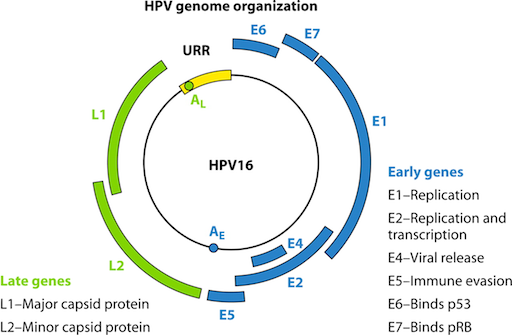
\includegraphics[scale=0.7]{IMG/genoma.png}
	\caption{Cartoon illustrating the genomic organization of a typical mucosal high-risk HPV. The genome contains early and late regions (E), which relate to the positions of the genes within the genome and their timing of expression during the viral life cycle. The early region carries a number of genes which function at the level of viral replication and transcription, i.e., E2, E1, E6, and E7. E2 encodes a protein which has an auxiliary role in viral replication and also functions at the level of transcriptional regulation of the viral early genes. The E6 and E7 genes encode the major transforming proteins of the oncogenic HPVs. The late region (L) encodes viral structural proteins, with L1 being the major capsid protein and L2 being the minor capsid protein.}
	\label{genoma}
\end{figure}
%doi: 10.1128/CMR.05028-11 Clin. Microbiol. Rev. April 2012 vol. 25 no. 2 215-222 1 April 2012

%Foto del HPV-16 con Cryo-EM (nobel química 2017)

The finding was followed by epidemiologists, molecular biologists, vaccinologists, and clinicians culminating in 2006 with the development of effective prophylactic vaccines for human papillomavirus, which have the means to prevent 70-80\% of cervical cancer. Zur Hausen was awarded the Nobel Prize in Physiology or Medicine in 2008, in recognition of his discovery.

\begin{figure}[ht]
	\centering
	
\includegraphics[scale=0.7]{IMG/zurHausen.png}
	\caption{Harald zur Hausen (born 11 March 1936) is a German virologist and professor emeritus. He has done research on cancer of the cervix, where he discovered the role of papilloma viruses, for which he received the Nobel Prize in Physiology or Medicine 2008.}
	\label{zurHausen}
\end{figure} 
%Foto de Zur Hausen

%Datos de lo malo que es
HPV types are often referred to as low risk (LR) wart causing or high risk (HR) cancer causing, based on whether they put a person at risk for cancer.  The types of HPV that can cause genital warts are not the same as the types that can cause cancer.
Persistent human papillomavirus (HPV) infections with genotypes 16 and 18 are responsible for about 70\% of all cervical cancer 
%Clifford GM, Rana RK, Franceschi S, Smith JS, Gough G, Pimenta JM. Human papillomavirus genotype distribution in low-grade cervical lesions: comparison by geographic region and with cervical cancer. Cancer Epidemiol Biomarkers Prev. 2005;14:1157–1164. doi: 10.1158/1055-9965.EPI-04-0812.
%Munoz N, Bosch FX, de Sanjosé S, Herrero R, Castellsague X, Shah KV, et al. Epidemiologic classification of human papillomavirus types associated with cervical cancer. N Engl J Med. 2003;348:518–527. doi: 10.1056/NEJMoa021641.
, with 40-85\% of other anogenital cancers: anal, penile, vaginal, and vulvar cancer, and also 16-28\% of the head and neck cancers.
%%WHO International Agency for Research on Cancer. IARC Monographs on the Evaluation of Carcinogenic Risk to Humans. Human Papillomavirusses. Volume 90. 2007.
%https://www.ncbi.nlm.nih.gov/pmc/articles/PMC4331443/

HPV is a cause of other non malignant diseases, to mention genotypes 6 and 11 cause about 90\% of anogenital warts, and secondarily juvenile onset of recurrent respiratory papillomatosis.
%Lacey CJ, Lowndes CM, Shah KV. Chapter 4: Burden and management of non-cancerous HPV-related conditions: HPV-6/11 disease. Vaccine. 2006;24(Suppl 3):S35–S41. doi: 10.1016/j.vaccine.2006.06.015.

% Literatura dura
Genital human papillomavirus (HPV) is the most common sexually transmitted infection in the United States. More than 40 HPV types can infect the genital areas of men and women, including the skin of the penis, vulva (area outside the vagina), and anus, and the linings of the vagina, cervix, and rectum. These types can also infect the lining of the mouth and throat.

\begin{figure}[ht]
	\centering
	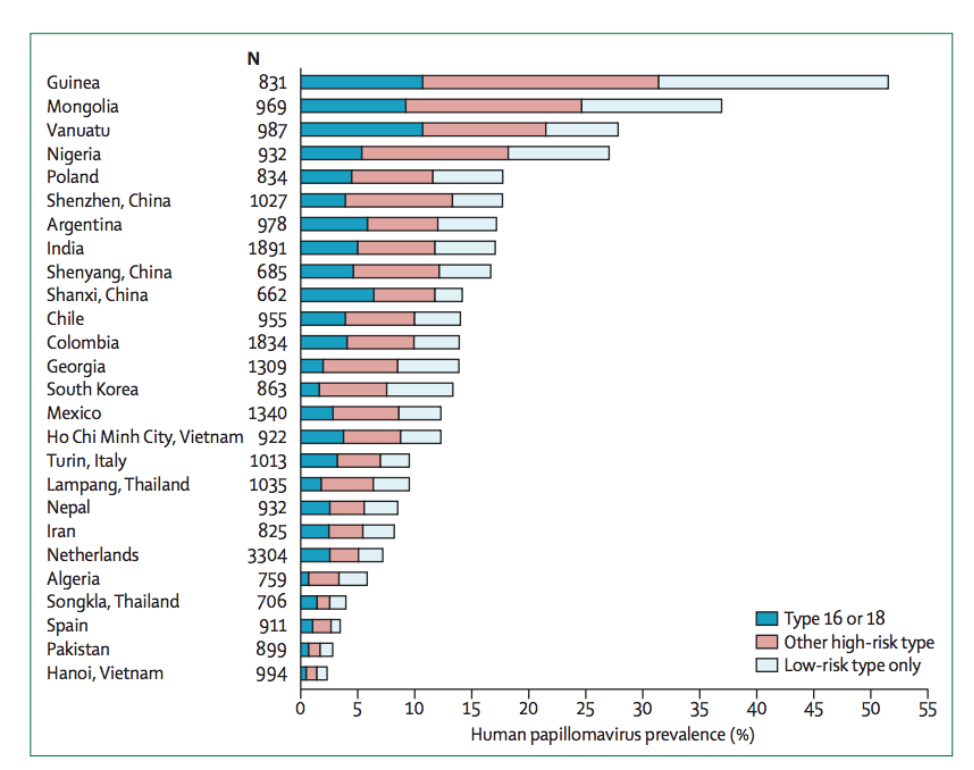
\includegraphics[scale=0.7]{IMG/prevalence.png}
	\caption{Age\-adjusted prevalence of cervical human papillomavirus DNA in sexually active women aged 15\-69 years. Data are from IARC Prevalence Surveys, 1990\-2012.4}
	\label{zurHausen}
\end{figure} 
%Foto de prevalencia


%Literatura
Most people who become infected with HPV do not know they have it. Usually, the body's immune system gets rid of the HPV infection naturally within two years. This is true of both HR and LR types. By age 50, at least 4 out of every 5 women will have been infected with HPV at one point in their lives. HPV is also very common in men, and often has no symptoms.

When the body's immune system can't get rid of a HR HPV infection, it can linger over time and turn normal cells into abnormal cells and then cancer. About 10\% of women with HR HPV on their cervix will develop long-lasting HPV infections that put them at risk for cervical cancer. Similarly, when HR HPV lingers and infects the cells of the vulva, vagina, penis, anus, or the oropharynx (back of the throat, including the base of the tongue and tonsils), it can cause cell changes called precancers. These may eventually develop into cancer if they're not found and removed in time. These cancers are much less common than cervical cancer. Much less is known about how many people with HPV will develop cancer in these areas.

%Empiezo con las vacunas
\section{Vaccines}
Since the release of the first vaccines in 2006, nowadays there are three available: a quadrivalent (including HPV genotypes 16, 18, 6 and 11) and a bivalent vaccine (including genotypes 16 and 18) and a nonavalent (including genotypes 6, 11, 16, 18, 31, 33, 45, 52 and 58). All vaccines are efficacious to protect against precancerous lesions in the cervix, vulva or vagina; in addition, the quadrivalent and nonavalent prevent precancerous anal lesions, anal cancer and anogenital warts.

\begin{figure}[ht]
	\centering
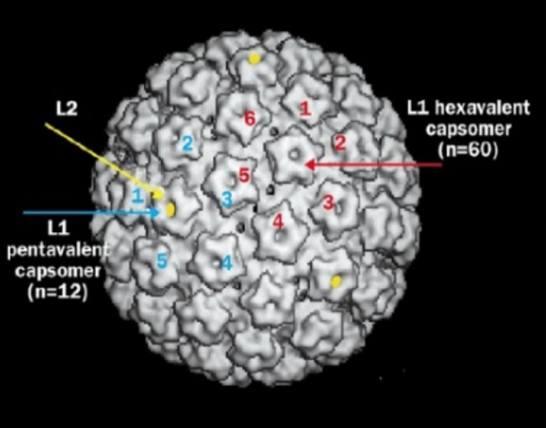
\includegraphics[scale=0.7]{IMG/cryo.png}
\caption{Structure of a HPV virus-like particle. A three-dimensional reconstruction of a cryolectron micrograph (cryo-EM) of a virus-like particle (VLP) is shown. The VLP is composed of 60 hexavalent capsomers and 12 pentavalent capsomers, all consisting of pentamers of L1 protein. The L2 protein is not visible by cryo-EM but is tought to be associated with the pentavalent capsomers, and have been colored in yellow.}
\label{cryo}
\end{figure}  

According to the Advisory Committee on Immunization Practices (ACIP) from the Centers for Disease Control (CDC) and Prevention, new recommendations are given for use of a 2-dose schedule for girls and boys who initiate the vaccination series at ages 9 through 14 years. Three doses remain recommended for persons who initiate the vaccination series at ages 15 through 26 years and for immunocompromised persons.

In Spain HPV vaccine is given to adolescent girls as part of the national immunization programme, and is recommended at different age groups in different Autonomous Communities. Numerous cost-effectiveness studies of HPV-vaccination have been published in other countries. However, few studies include the prophylactic effect of all HPV-associated diseases, or the impact of vaccinating men.

There are countries that recommend also vaccinating boys in order to decrease the burden of disease in them. Some models have shown that the female vaccination program has some herd immunity and the impact of implementing the vaccination in males may not be cost effective, however not vaccinating males leaves them at risk of cancers, especially the groups that do not benefit of the herd immunity, as the males that have sex with males.
Besides, there is no economic analysis of the nonavalent program in Spain, and it is important from the decision making perspective.

Even with the high prevalence of sexually transmitted diseases there are few studies devoted to ascertain the structure of sexual networks and its role in disease transmission. Most studies are restricted to small communities such as the Jefferson High Schools project (P. S. Bearman et al., Chains of Affection: The Structure of Adolescent Romantic and Sexual Networks, American Journal of Sociology, 110(1) (2004) 44-91) or that of Likoma Island (S. Helleringer and H. P. Kohler, Sexual network structure and the spread of HIV in Africa: evidence from Likoma Island, Malawi, AIDS 21 (2007) 2323-2332).

Random network mathematical models may simulate the interactions and propagations of all these viruses through sexual contacts among a population of more than one million people (including heterosexual and homosexual populations). As this model is based upon a network instead of traditional continuous model approaches (E. H. Elbasha et al., Model for assessing human papillomavirus vaccination strategies,  Emerging. Inf. Dis.  2007; 13:28-41) we will be able to determine with higher accuracy the effect of vaccination in a short and large periods of time.

The Human papillomaviruses HPV vaccine induces a herd immunity effect in genital warts when a large number of the population is vaccinated. This aspect should be taken into account when devising new vaccine strategies, like vaccination at older ages or male vaccination. Therefore, it is important to develop mathematical models with good predictive capacities. We devised a sexual contact network that was calibrated to simulate the Spanish epidemiology of different HPV genotypes. Through this model, we simulated the scenario that occurred in Australia in 2007, where 12-13 year-old girls were vaccinated with a three-dose schedule of a vaccine containing genotypes 6 and 11, which protect against genital warts, and also a catch-up program in women up to 26 years of age. Vaccine coverage were $73\%$ in girls with three doses and with coverage rates decreasing with age until $52\%$ for 20-26 year-olds. A fast $59\%$ reduction in the genital warts diagnoses occurred in the model in the first years after the start of the program, similar to what was described in the literature.




%
\chapter{A first mathematical model of the evolution of the Basque Country population respect to their opinion about ETA under its pressure}\label{paper1}

In this chapter, our objective is to state a first type-epidemiological mathematical model. This model study the evolution over the time of populations in the Basque Country respect their opinions about the ETA's goals. This way, as we mentioned in Section \ref{reduccion}, we want to focus on the evolution of the supporters of ETA's goals to see if they decrease or not.

Here, we recall that popular support is an important enabler for radical violent organizations and it may be crucial for their survival and these extremist groups have also an impact in the societies where they are inserted, especially if those groups are engaged in violent activities. 

The democratic system in the Basque Country and in the rest of Spain is affected by terrorist acts of ETA (murders, kidnapping, vandalism, etc.). Thus, terrorism uses to be one of the most important topics for Spanish public opinion.

In order to carry out this study, the Basque Country' population will be divided into people that:

\begin{itemize}
\item agree with ETA in the objective of independence and the use of
violence to get it,
\item agree with ETA only in the objective of independence, without the use
of violence,
\item completely disagree with ETA.
\end{itemize}

Then, from electoral manifestos and using statistical techniques, in Section \ref{1.1}, a classification of different political parties respect to the political goal "independence" is done. This allows us to divide the Basque population depending on their support to ETA's goals. In Section \ref{1.2} a type-epidemiological mathematical model where the pressure of ETA and its related groups affects the opinion of the people about the support of ETA's goals, is proposed. The model developed in Section \ref{1.2} is not appropriate for data obtained in Section \ref{1.1} (same units), hence Section \ref{1.3} is devoted to scale the model properly to be fitted with classification data obtained in Section \ref{1.4}. Simulations to predict short- and medium-term evolution of population in the Basque Country deterministically and with uncertainty are presented in Section \ref{1.5}. Finally, Section \ref{1.6} is devoted to conclusions.

\section{Classification of ideological groups}\label{1.1}

Let us consider as source data the results of the general elections to the Spanish
Parliament in the Basque Country since June 15th 1977 to March 14th 2004 
\cite{mir}. Since 1977, 85 political parties nominated candidates to,
at least, one general election in the Basque Country electoral district.
General elections data have been considered because, in Spain, experts
consider that general elections give a more realistic political distribution
than local elections \cite{elecGen}.

Now, let us classify the parties with respect to their relation with the
political objective "independence". To do this, a survey is prepared to be
answered from the party's election manifestos. The survey consist of the following
questions (or ideological characteristics):

\begin{enumerate}
\item Nationalist (Yes/No),
\item Religious (Yes/No),
\item Supports violence (Yes/No),
\item Interventionist (Yes/No),
\item Ecologist (Yes/No),
\item Independence (Yes/No),
\item Ideology (right wing or center/left wing/nationalist).
\end{enumerate}

A non-parametric bivariant analysis \cite[Chap. 9]{Groot} is carried out
in order to determine the ideological characteristics (questions of the survey)
related to the use of the violence to get the independence.
These characteristics were "Independence", "Nationalism", "Ideology" and "Support violence"
with associated $p-$values less than $0.01$. In the multiple correspondence
analysis \cite[Chap. 10]{Hair} three different profiles can be seen (see
Figure \ref{1cluster}), nationalist parties agreeing with the independence and
the use of violence, right-wing and center parties against independence
and, in the middle of these profiles, left-wing parties with a non
homogeneous and/or ambiguous position respect to independence and the
use of violence.

\begin{figure}[htb]
\begin{center}
\includegraphics[scale=0.53]{IMG/1cluster.pdf}
\end{center}
\caption{Correspondence analysis shows three different profiles, nationalist 
parties, right-wing and center parties, and left-wing parties with ambiguous 
positions respect to independence and the use of violence.}
\label{1cluster}
\end{figure}

These three profiles (defined by the characteristics "Nationalist", "Independence" "Ideology" and "Support violence") lead us to do a non hierarchical cluster
analysis with three groups of parties, whose definition is determined by the
following characteristics:

\begin{itemize}
\item Group $G_{1}:$ non-nationalist parties against independence and the
use of the violence.
\item Group $G_{2}:$ nationalist parties agreeing with independence but
disagreeing with the use of the violence.
\item Group $G_{3}:$ nationalist parties agreeing with independence and the use
of the violence.
\end{itemize}

The above division of political parties allows us to classify the population depending on the parties they vote and the position of these parties respect to ETA's goals. With this approach, the population of the Basque Country can be divided into four subpopulations

\begin{itemize}
\item $E(t)$, number of people who share the common ideological
characteristics of parties in $G_{1}$ at time $t,$
\item $N(t)$, number of people who share the common ideological
characteristics of parties in $G_{2}$ at time $t,$
\item $V(t)$, number of people who share the common ideological
characteristics of parties in $G_{3}$ at time $t,$ and
\item $A(t)$, the rest of the people at time $t$. It includes
people who do not share the ideological characteristics of groups $G_{1},$ 
$G_{2}$ and $G_{3}$ or people who abstain.
\end{itemize}

Figure \ref{1graf1} shows the percentage of votes of each subpopulation in
each election. 

\begin{figure}[htb]
\begin{center}
\includegraphics[scale=0.62]{IMG/1datos.pdf}
\end{center}
\caption{This figure shows the percentage of votes of each subpopulation 
in each election. Vertical lines correspond to electoral days. Let us 
consider in our study data between $1979$ and $1996$, where most of the  
time the Socialist Party (PSOE) was in the government, and the same policy against terrorism can 
be assumed.}
\label{1graf1}
\end{figure}

Two considerations should be mentioned here to understand some trend changes in
Figure \ref{1graf1} at the beginning and at the end. The general elections in
1977 were the first celebrated after the dictator Franco died. Lots of
parties presented candidates, the political situation was not clear and it
is reflected in the data. In 2000, political parties in group $G_{3}$ asked abstention and in $2004$, the "Law of Political Parties" (LPP) forbade these parties from nominating candidates. In fact, LPP outlawed the political parties that did not condemn the violence. Notice that in $2000$ and $2004$ abstention increased, but this was because the votes for parties of group $G_{3}$ were considered void, increasing the subpopulation $A\left( t\right)$.

All the above leads us to consider only election data since 1979 to 1996
where the major part of time the Socialist Party (PSOE) governed Spain and
the same policy against terrorism can be assumed in order to fit the
model we will develop in Section \ref{1.2}.

\begin{table}[htb]
\label{1Table1}
\begin{center}
\begin{tabular}{ccccc}
\hline
Election date & $E(t)$ & $N(t)$ & $V(t)$ & $A(t)$ \\ \hline
\multicolumn{1}{l}{Jun 15th, 1977} & \multicolumn{1}{l}{$0.435392$} & 
\multicolumn{1}{l}{$0.266825$} & \multicolumn{1}{l}{$0.0316636$} & 
\multicolumn{1}{l}{$0.26612$} \\ 
\multicolumn{1}{l}{Mar 1st, 1979} & \multicolumn{1}{l}{$0.278466$} & 
\multicolumn{1}{l}{$0.233303$} & \multicolumn{1}{l}{$0.0967287$} & 
\multicolumn{1}{l}{$0.391502$} \\ 
\multicolumn{1}{l}{Oct 28th, 1982} & \multicolumn{1}{l}{$0.347978$} & 
\multicolumn{1}{l}{$0.306366$} & \multicolumn{1}{l}{$0.114331$} & 
\multicolumn{1}{l}{$0.231325$} \\ 
\multicolumn{1}{l}{Jun 22nd, 1986} & \multicolumn{1}{l}{$0.294959$} & 
\multicolumn{1}{l}{$0.245271$} & \multicolumn{1}{l}{$0.117587$} & 
\multicolumn{1}{l}{$0.342183$} \\ 
\multicolumn{1}{l}{Dec 17th, 1989} & \multicolumn{1}{l}{$0.246631$} & 
\multicolumn{1}{l}{$0.283516$} & \multicolumn{1}{l}{$0.111871$} & 
\multicolumn{1}{l}{$0.357982$} \\ 
\multicolumn{1}{l}{Jun 6th, 1993} & \multicolumn{1}{l}{$0.330461$} & 
\multicolumn{1}{l}{$0.234575$} & \multicolumn{1}{l}{$0.100969$} & 
\multicolumn{1}{l}{$0.333994$} \\ 
\multicolumn{1}{l}{Mar 3rd, 1996} & \multicolumn{1}{l}{$0.364871$} & 
\multicolumn{1}{l}{$0.236203$} & \multicolumn{1}{l}{$0.0872077$} & 
\multicolumn{1}{l}{$0.311718$} \\ 
\multicolumn{1}{l}{Mar 12th, 2000} & \multicolumn{1}{l}{$0.364974$} & 
\multicolumn{1}{l}{$0.239676$} & \multicolumn{1}{l}{$0.$} & 
\multicolumn{1}{l}{$0.39535$} \\ 
\multicolumn{1}{l}{Mar 14th, 2004} & \multicolumn{1}{l}{$0.382756$} & 
\multicolumn{1}{l}{$0.299592$} & \multicolumn{1}{l}{$0.$} & 
\multicolumn{1}{l}{$0.317652$} \\ \hline
\end{tabular}
\end{center}
\caption{Data corresponding to graphic in Figure \ref{1graf1}.}
\end{table}

Taking into account that, in Spain, only people older than $18$ can vote and
supposing that children and teenagers have the same way of thinking as their
parents, let us assume that data in Table \ref{1Table1} gives a general voting distribution 
of the whole population in the Basque Country, and taking into account the classification of parties, 
the distribution of the people depending on their support to ETA's goals.

\section{Building the type-epidemiological mathematical model}\label{1.2}

Let us consider the population of the Basque Country divided into four
subpopulations determined in Section \ref{1.1}, that is, $E,$ $N,$ 
$V$ and $A$. Also, we assume that:

\begin{itemize}
\item The number of births $\Lambda(t)$ and the number of
deaths $\Phi(t)$ in the year $t$, are proportional to the number of individuals
in each subpopulation.

\item Terrorism does not increase substantially the number of deaths. 

\item The immigration $\Gamma(t)$ and emigration $\Sigma(t)$ in Basque Country 
are also included. It is considered that immigration and emigration only occurs 
in subpopulations $E$ and $A$ due to the terror pressure \cite{exilio2, exilio3, exilio1} 
in proportions $\alpha_{1}$ and $\alpha_{2}$, respectively, to be determined.
\end{itemize}

In order to determine the rest of transition terms, 
partial correlation coefficients have been used. This coefficient studies
the linear relation between two variables under the influence of a third
variable \cite{Groot}. To carry out this study, let us take data of Table
\ref{1Table1} corresponding to elections from March 1st 1979 to March 3rd
1996.

The partial correlation coefficient between subpopulations $E$ and $A$ under
the influence of $V$ is $-0.8409$ with a $p-$value of $0.009$ ($p-value < 0.05$). It means that
there is a linear inverse relation between $E$ and $A$ under $V,$ that is,
under $V$ an increasing of subpopulation $E$ implies a decrease of
subpopulation $A$ and vice versa. Moreover, the linear correlation
coefficient between $E$ and $A$ without the presence of $V$ is not
significant. Therefore the transition between $E$ and $A$ is not linear because it is only possible under the influence of population $V$, and it is modeled by the nonlinear term

\[
\beta_{1} E(t) \frac{V(t)}{T(t)}, 
\]

where $\beta_{1} > 0$ indicates that the transition is due to the pressure of
violent acts and $\beta_{1} < 0$ indicates a law enforcement.

Analogously, a similar situation occurs between subpopulations $A$ and $V$
under the pressure of $V$. Then, the transition between subpopulations $A$
and $V$ is modeled by the nonlinear term

\[
k \beta_{1} A(t) \frac{V(t)}{T(t)}, 
\]

with $k > 0$.

On the other hand, the partial correlation coefficient between
subpopulations $N$ and $A$ under the influence of $E$ is $-0.6292$ with a 
$p- $value of $0.05$ and there is a linear inverse relation between $N$ and 
$A $ under $E$. Also, the linear correlation coefficient between $N$ and $A$
without the presence of $E$ is not significant. Therefore the transition
between $N$ and $A$ is modeled by the nonlinear term

\[
\beta_{2} N(t) \frac{E(t)}{T(t)}. 
\]

Then, the system of differential equations that models the evolution over the time of populations in the Basque Country respect their opinions about the ETA's goals under the pressure of its violence is given by

\begin{eqnarray}
E'(t)	& = &	\Lambda(t) E(t) + \alpha_{2} \Gamma(t) - \beta_{1} E(t) \frac{V(t)}{T(t)} - \label{1m1} \\
        &   &	\Phi(t) E(t) - \alpha_{1} \Sigma(t),  \nonumber \\                          
N'(t)	& = &	\Lambda(t) N(t) - \beta_{2} N(t) \frac{E(t)}{T(t)} - \Phi(t) N(t),  \label{1m2} \\
V'(t)	& = &	\Lambda(t) V(t) + k \beta_{1} A(t) \frac{V(t)}{T(t)} - \Phi(t) V(t),  \label{1m3} \\
A'(t)	& = &  	\Lambda(t) A(t) + (1 - \alpha_{2}) \Gamma(t) + \beta_{1} E(t) \frac{V(t)}{T(t)} + \label{1m4} \\
		&   &	\beta_{2}N(t) \frac{E(t)}{T(t)} - k \beta_{1} A(t) \frac{V(t)}{T(t)} - \Phi(t) A(t) - 
		        (1 - \alpha_{1}) \Sigma(t),  \nonumber \\
T(t)		& = &	E(t) + N(t) + V(t) + A(t).  \label{1m5}
\end{eqnarray}

The above system of differential equations can be represented by the diagram of Figure \ref{1diagrama}.

\begin{figure}[htb]
\begin{center}
\includegraphics[scale=0.48]{IMG/1DiagramaModeloFanatismo.pdf}
\end{center}
\caption{Diagram corresponding to the model defined by the system of 
differential equations $\left( \protect\ref{1m1}\right) -\left( \protect\ref{1m5}\right).$}
\label{1diagrama}
\end{figure}

\section{Scaling the model $(\ref{1m1}) -(\ref{1m5})$}\label{1.3}

Data obtained in Section \ref{1.1} is related to the percentages of
population while model $\left( \ref{1m1}\right) -\left( \ref{1m5}\right)$
is related to the number of individuals. It leads us to transform (by scaling) the
model into the same units as data, because one of our objectives is to fit the
data with the model in next section.

Hence, following ideas developed in \cite{Martcheva, Mena, scaling} about how
to scale models where the population is varying in size, adding equations 
$\left( \ref{1m1}\right) -\left( \ref{1m4}\right)$ it is obtained

\begin{equation}
T^{\prime }\left( t\right) =\left[ \Lambda \left( t\right) -\Phi \left(
t\right) \right] T\left( t\right) +\Gamma \left( t\right) -\Sigma \left(
t\right).  \label{1eqT}
\end{equation}

Dividing both members of $\left( \ref{1eqT}\right) $ by $T\left( t\right) $
we have that

\begin{equation}
\frac{T^{\prime }\left( t\right) }{T\left( t\right) }=\Lambda \left(
t\right) -\Phi \left( t\right) +\frac{\Gamma \left( t\right) -\Sigma \left(
t\right) }{T\left( t\right) }.  \label{1T/T}
\end{equation}

On the one hand, if we define the rates (depending on time)

\begin{equation}
e=\frac{E}{T},n=\frac{N}{T},v=\frac{V}{T},a=\frac{A}{T},\gamma =\frac{\Gamma 
}{T},\sigma =\frac{\Sigma }{T},  \label{1ratios}
\end{equation}

equation $\left( \ref{1T/T}\right) $ can be transformed into

\begin{equation}
\frac{T^{\prime }}{T}=\Lambda -\Phi +\gamma -\sigma .  \label{1T/Tcorta}
\end{equation}

On the other hand, let us compute the derivative of $e,$ defined in 
$\left(\ref{1ratios}\right).$ Using $\left(\ref{1T/Tcorta}\right)$ we obtain that,

\begin{equation}
e^{\prime }=\frac{E^{\prime }T-ET^{\prime }}{T^{2}}=\frac{E^{\prime }}{T}-
\frac{E}{T}\frac{T^{\prime }}{T}=\frac{E^{\prime }}{T}-e\left[ \Lambda -\Phi
+\gamma -\sigma \right] .  \label{1chulla}
\end{equation}

In an analogous way, we also have that,

\begin{eqnarray*}
n^{\prime } &=&\frac{N^{\prime }}{T}-n\left[ \Lambda -\Phi +\gamma -\sigma 
\right] , \\
v^{\prime } &=&\frac{V^{\prime }}{T}-v\left[ \Lambda -\Phi +\gamma -\sigma 
\right] , \\
a^{\prime } &=&\frac{A^{\prime }}{T}-a\left[ \Lambda -\Phi +\gamma -\sigma 
\right] .
\end{eqnarray*}

Now, consider equation $\left( \ref{1m1}\right) .$ If we divide it by $T,$ we
have

\[
\frac{E^{\prime }}{T}=\Lambda \frac{E}{T}+\alpha _{2}\frac{\Gamma }{T}-\beta
_{1}\frac{E}{T}\frac{V}{T}-\Phi \frac{E}{T}-\alpha _{1}\frac{\Sigma }{T}, 
\]

using $\left( \ref{1chulla}\right) $ and substituting by the corresponding
rates defined in $\left( \ref{1ratios}\right) $ one gets 

\[
e^{\prime }+e\left[ \Lambda -\Phi +\gamma -\sigma \right] =\Lambda e+\alpha
_{2}\gamma -\beta _{1}ev-\Phi e-\alpha _{1}\sigma , 
\]

obtaining the scaled equation

\begin{equation}
e^{\prime }=\left( \sigma -\gamma \right) e+\alpha _{2}\gamma -\beta
_{1}ev-\alpha _{1}\sigma .  \label{1sm1}
\end{equation}

The remaining equations can be scaled in the same way to obtain

\begin{eqnarray}
n^{\prime } &=&\left( \sigma -\gamma \right) n-\beta _{2}ne,  \label{1sm2} \\
v^{\prime } &=&\left( \sigma -\gamma \right) v+k\beta _{1}av,  \label{1sm3} \\
a^{\prime } &=&\left( \sigma -\gamma \right) a+\left( 1-\alpha _{2}\right)\gamma +\beta _{1}ev+ \label{1sm4} \\
            & &\beta _{2}ne-k\beta _{1}av-\left( 1-\alpha _{1}\right) \sigma. \nonumber 
\end{eqnarray}

Notice that the scaled system of differential equations $\left( \ref{1sm1}
\right) -\left( \ref{1sm4}\right) $ is also a non-autonomous system because
the immigration $\left( \gamma \right) $ and emigration $\left( \sigma
\right) $ rates depend on time.

\section{Model fitting}\label{1.4}

Taking data in Table \ref{1Table1} corresponding to elections from March 1st
1979 to March 3rd 1996, let us to fit data with the scaled model 
$\left( \ref{1sm1}\right) -\left( \ref{1sm4}\right).$

Moreover demographic data from \cite{demogPV}, in particular annual
population, immigration and emigration data in the interval 1979 to 1996 are
considered. Hence, in order to compute immigration and emigration rate
functions $\gamma \left( t\right) $ and $\sigma \left( t\right),$ we divide
each immigration and emigration datum by the corresponding population datum.
Then, we use piecewise linear interpolation to construct both functions, $\gamma$ and 
$\sigma $. Migration data are depicted in Figure \ref{1migra}.

\begin{figure}[htb]
\begin{center}
\includegraphics[scale=0.8]{IMG/1migracion.pdf}
\end{center}
\caption{Immigration and emigration rates from 1979 until 2015. Notice that from 2005 these rates are constant, equal to the ones in 2005.}
\label{1migra}
\end{figure} 

As initial condition of the model $\left( \ref{1sm1}\right) -\left(\ref{1sm4}\right),$ 
it is considered

\begin{equation}
\begin{array}{cc}
E\left( t_{0}\right) =0.278466, & N\left( t_{0}\right) =0.233303, \\ 
V\left( t_{0}\right) =0.0967287, & A\left( t_{0}\right) =0.391502,
\end{array}
\label{1IC}
\end{equation}

where $t_{0}$ corresponds to March 1st 1979 (see Table \ref{1Table1}). In
order to compute the best fitting, we carried out computations with 
\emph{Mathematica} \cite{Wolfram} and we implemented the function

\[
\begin{array}{ccccc}
\mathbb{F} & : & \mathbb{R}^{5} & \longrightarrow & \mathbb{R} \\ 
&  & \left( \beta _{1},\beta _{2},k,\alpha _{1},\alpha _{2}\right) & 
\longrightarrow & \mathbb{F}\left( \beta _{1},\beta _{2},k,\alpha
_{1},\alpha _{2}\right)
\end{array}
\]

which variables are $\beta _{1},$ $\beta _{2},$ $k,$ $\alpha _{1}$ and 
$\alpha _{2}$ such that:

\begin{enumerate}
\item Solve numerically (using \textit{Mathematica} command \emph{NDSolve[]}) the system of differential
equations $\left( \ref{1sm1}\right) -\left( \ref{1sm4}\right) $ with initial
values $\left( \ref{1IC}\right),$

\item For $t=$ Oct 28th 1982, Jun 22nd 1986, Dec 17th 1989, Jun 6th 1993 and
Mar 3rd 1996, corresponding to election days, evaluate the computed
numerical solution for each subpopulation $E\left( t\right) ,$ $N\left(
t\right) ,$ $V\left( t\right) ,$ $A\left( t\right) $.

\item Compute the mean square error between the values obtained in Step 2
and the electoral data from Oct 28th 1982 to Mar 3rd 1996, (Table 
\ref{1Table1}).
\end{enumerate}

Function $\mathbb{F}$ takes values in $\mathbb{R}^{5}$ ($\beta _{1},$ 
$\beta_{2},$ $k,$ $\alpha _{1}$ and $\alpha _{2})$ and returns a positive real
number. Hence, we minimize this function using the Nelder-Mead
algorithm \cite{Nelder, Press}, that does not need the computation of
any derivative or gradient, which is impossible to know in this case. Thus, the values of $\beta _{1},$ $\beta _{2},$ $k,$ 
$\alpha _{1}$ and $\alpha _{2},$ with restrictions $0\leq \alpha _{1},\alpha_{2}\leq 1$ and $k>0,$ that minimize the function $\mathbb{F}$ are

\begin{equation}
\begin{array}{l}
\beta_{1}=0.0534,\ \beta_{2}=-0.0338,\\
 k=0.5352,\\
\alpha_{1}=0.8945,\ \alpha_{2}=0.9999.  
\end{array}
\label{1parametros}
\end{equation}

Parameters indicate that population flows from $E$ to $A$ and from $A$ to $V$ ($\beta_{1}, k > 0$), and from $A$ to $N$ ($\beta_{2} < 0$) very slowly. Furthermore, the value of $k$ indicates that the pressure of $V$ affects twice to $E$ than to $A$. Additionally, almost all emigration and immigration occurs in subpopulation $E$ ($\alpha_{1}=0.8945$, $\alpha_{2}=0.9999$). 

\section{Trends over next few years}\label{1.5}

Once the model parameters have been estimated, under the assumption that government anti-terrorist policies and ETA strategies do not change, we can use the model to predict the trend of each subpopulation until $2020$, i.e., the deterministic prediction. To do so, demographic data from \cite{demogPV} are used: immigration and emigration available data go from 1977 until 2008 and the 2008 datum is repeated until 2020; real population data from 1975 to 2008 are available and also predictions until 2020. 

Then, we use the model parameters obtained in (\ref{1parametros}), substitute them into the model and obtain the model forecasting for next electoral years $2012$, $2016$ and $2020$. The results can be seen in Table \ref{1Table2}.

\begin{table}[ht]
\begin{center}
\begin{tabular}{c|cccc}
  &  $E$ & $N$ & $V$ & $A$ \\
 \hline    
\begin{tabular}{l}
 $2012$ \\  $2016$\\  $2020$
\end{tabular}
&  
\begin{tabular}{c}
  0.343714 \\ 0.359023 \\ 0.373446
\end{tabular}
 & 
\begin{tabular}{c}
  0.291674\\	0.296761	\\ 0.302587
\end{tabular}
 & 
\begin{tabular}{c}
  0.114067 \\ 0.113756 \\	0.113205
\end{tabular}
& 
\begin{tabular}{c}
  0.250546\\	0.23046\\0.210763
\end{tabular}
\end{tabular}
\end{center}
\caption{Deterministic prediction for the next electoral years $2012$, $2016$ and $2020$. } 
\label{1Table2}
\end{table}

Looking at Tables \ref{1Table1} (data from $1979$ to $1996$) and \ref{1Table2} jointly, we can observe a slight increase in groups $E$, $N$ and $V$ at the expense of $A$. It is noteworthy to see how subpopulation $V$ has hardly varied during the 40 years studied. 

However, as we mentioned in the Introduction chapter, uncertainty is a key part dealing with Social Sciences phenomena. Therefore, the supposition that parameters always remain constant or data in Table \ref{1Table1} and demographic data do not contain errors, is not appropriate. Thus, it is natural to consider that the model parameters $\beta_{1}$, $\beta_{2}$, $k$, $\alpha_{1}$ and $\alpha_{2}$ contain uncertainties. Hence, the deterministic prediction can give us an idea about future trends but, in this case, the obtained values may not be accurate.

Therefore, we propose forecasting future trends using confidence intervals. In order to calculate these confidence intervals, let us use the technique called Latin Hypercube Sampling (LHS) to vary parameter values in the proposed model. LHS, a type of stratified Monte Carlo sampling, is a sophisticated and efficient method for achieving equitable sampling of all input parameters simultaneously \cite{BLOWER, OLSSON}. Each parameter for a model can be defined as having an appropriate probability density function associated with it. It is usual to use the uniform distribution centred at deterministic parameter estimators in absence of data to give information as to the distribution for a given parameter \cite{MCKAY, OLSSON}. Thus, the model can be simulated by sampling a single value from each parameter distribution. Many samples should be taken and many simulations should be run, producing variable output values that can be treated with descriptive statistic techniques to compute the means and $90\%$ confidence intervals.

An important issue arises here and it is how much we should vary the parameters to quantify uncertainty. Some studies analyse the effect on populations of health campaigns \cite{SNYDER}, electoral campaigns \cite{FOURNIER} or the bombing attacks in Madrid few days before elections \cite{BALI}, and all of them over a short period. In these cases, what we call "effect" refers to a change of opinion to adopt a healthier way of life, to leave the abstention group and vote or to switch party. This change of opinion is about $5\%$ in health campaigns \cite{SNYDER}, $5\%-19\%$ in Canadian electoral campaigns depending on the time of decision \cite{FOURNIER} and around $10\%$ in the elections immediately after attacks in Madrid \cite{BALI}. Moreover, the referred changes are related to population, not to parameters and therefore, not related to rates of political ideology change. However, as we mentioned before, anti- or pro-terrorist policies and strategies are designed to change the value of the model parameters. Thus, even though we do not have any quantification of uncertainty in the parameters, let us assume that they may have a variation not greater than $20\%$ of their values, i.e., 

\begin{equation}
	\begin{array}{c}
		\beta_{1} \in [0.0428, 0.0642],\ \beta_{2} \in [-0.0270, -0.0406], \\ 
		\alpha_{1} \in [0.7156, 1],\ \alpha_{2} \in [0.78, 1].
	\end{array}
	\label{1int}
\end{equation}

Note that $20\%$ variation of $\beta_{1}$ implies $20\%$ variation of $k \beta_{1}$. Now, applying the LHS technique with $5,000$ samples using uniform distributions centred at the deterministic parameter values (\ref{1parametros}), i.e., for $5,000$ different $5-$tuples $(\beta_{1}, \beta_{2}, k, \alpha_{1}, \alpha_{2}),$ we solve the model to obtain $5,000$ outputs 

$$(E(t_f), N(t_f), V(t_f), A(t_f)),$$ 

for $t_f= 2012, 2016, 2020$, the coming electoral years. Hence, for each $t_f$ and for each subpopulation we can compute the $90\%$ confidence interval from the corresponding $5,000$ outputs. Results can be seen in Table \ref{1Table3}.

\begin{table}[ht]
\begin{center}
\begin{tabular}{c|cccc}
  &  $E$ & $N$ & $V$ & $A$ \\
 \hline
 $2012$	& $[0.261,0.37]$ & $[0.267,0.307]$ & $[0.109,0.124]$	 & $[0.217,0.345]$ \\
 $2016$	& $[0.266,0.387]$ & $[0.268,0.315]$ & $[0.108,0.125]$	 & $[0.196,0.337]$ \\
 $2020$	& $[0.271,0.404]$ & $[0.27,0.324]$ & $[0.107,0.126]$	 & $[0.173,0.33]$ 
\end{tabular}
\end{center}
\caption{$90\%$ confidence intervals obtained with $5,000$ model outputs using LHS technique in the next electoral years $2012$, $2016$ and $2020$. } 
\label{1Table3}
\end{table}

The results obtained in the present section are summarised in Figure \ref{1ajuste}. The parts of each graph are: 

\begin{itemize}
\item the points on the left are data from Table \ref{1Table1}; 
\item the continuous line is the deterministic model output for parameters in (\ref{1parametros}); 
\item the $90\%$ confidence intervals in $2012$, $2016$ and $2020$ are on the right; 
\item the points in the middle of the confidence intervals are the mean of $5,000$ outputs for each subpopulation and each electoral year.
\end{itemize}

\begin{figure}[htb]
\includegraphics[scale=0.8]{IMG/1AjustePrediccionCI.pdf}
\caption{Model fitting since March 1st 1979 to March 3rd 1996 and future prediction for each subpopulation, $E,$ $N,$ $V$ and $A.$ Points on the left are data of election days, the continuous lines the solution of the model until 2020. The $90\%$ confidence intervals for electoral years with their mean are on the right.}
\label{1ajuste}
\end{figure}

Figure \ref{1ajuste} allows us to say, on the one hand, that $E$ and $A$ are the ideological groups with more uncertainty, $10.9\%-13.3\%$ and  $12.5\%-15.6\%$ respectively (maximum and minimum length of their respective confidence intervals in Table \ref{1Table3}), where the deterministic prediction is far from the mean of the confidence intervals. This brings up some doubts as to the deterministic prediction, to consider more conservative predictions than the one obtained with LHS one and to point out the high sensitivity of groups $E$ and $A$ to model parameter perturbations (policy changes). On the other hand, subpopulations $N$ and $V$ have few uncertainty, $4\%-5.4\%$ and $1.5\%-1.9\%$ respectively, and the deterministic prediction is very close to the mean of confidence intervals. This leads us to say that there is a minor flow across groups $V$ and $N$. Even though the confidence interval variations are greater than the ones in $V$, the population in $N$ is almost three times the one in $V$ and the variation $4\%-5.4\%$ of $N$ is less than three times the one of $V$. It also suggests that subpopulations $N$ and $V$ are less sensitive to model parameter perturbations (policy changes).

\section{Conclusions}\label{1.6}

In this chapter, we propose a type-epidemiological model to analyse the evolution over the time of populations in the Basque Country respect their opinions about the ETA's goals, taking into account that ETA uses violence to demand Basque independence from Spain. 

Using this model and applying the Latin Hypercube Sampling, we predict ideological trends over the next few years giving $90\%$ confidence intervals. The application of LHS is our first approach in dealing with model uncertainty, but in this case with an important drawback as is the quantification of the variation of the model parameters and the probability distribution they follow. We will attempt to overcome these inconveniences in the following chapters.

\textbf{Remark.} As we mentioned in the Introduction chapter, a paper including some results presented in this chapter was rejected to be published. One of the main drawbacks mentioned was related to the division into subpopulations, because the division was not well done and as a consequence, the predictions given in Table \ref{1Table3} are far to be correct. For instance, we predict a result of $10.9\% - 12.4\%$ for parties in $V$ for elections in year 2012 and, as we said in Chapter \ref{ETA} the parties included in $V$ obtained around $25\%$ of votes, being the second most voted parties in the Basque Country. Moreover, an electoral prediction over the next three election dates ($12$ years) may be considered too long. 

Therefore, although the model presented here was well considered by some referees and colleagues, it is only a rough approach to the problem. This is an example of the difficulty of modelling in Social Sciences.

However, we contacted with an expert who addressed our work and this is reflected in the following chapters.


\chapter{Australian Model}\label{introAustralia}

\section{Introduction}
Human papillomaviruses (HPV) encompass more than $100$ genotypes of viruses that infect cutaneous, genital and respiratory epithelia of humans worldwide. These are divided into high risk (HR), those that are directly related to the origin of cancers, and low risk (LR) genotypes that provoke mucocutaneous lesions. HPV $16$ and $18$ are responsible for about $70\%$ of cervical cancers, and different proportion of other malignancies: vaginal, anal, mouth and throat, etc.
HPV $6$ and $11$ are responsible for over $90\%$ of genital warts (GW). High risk genotypes are the direct cause of clinically important diseases such as cervical carcinoma associated with oncoviruses HPV $16$ and $18$. In recent years, about 500,000 new cases were diagnosed annually and 200,000 women died as a consequence of the progression of cervical dysplasias to invasive carcinomas \cite{Pathology}.

HPV is the most common sexually transmitted infection (STI) in the world. It is estimated that about 1 million new cases of GW are reported each year and the cost of treatment is increased by the tendency of these warts to recur after initial clearance. The cost of the treatment of genital warts was estimated to exceed \$ $3.8$ billion in the U.S. in $1997$ \cite{Roberts}. In Spain, there were 35,000 cases in women in $2007$ with an overall annual cost of \euro \ $47$ million \cite{CLEOPATRE}.

Two vaccines consisting of non-infectious HPV virus-like particles (VLP) \cite{McNeil} containing the capsid protein L1 of the virus but not the viral DNA. They induce a high immune response and prevent premalignant lesions. Both vaccines contain genotypes $16$ and $18$, and one of them adds VLP against genotypes $6$ and $11$ (HPV4).

In the Region of Valencia, Spain, the vaccine is administered to girls aged $15$ years old or less. Similar vaccination strategies of this kind were modelled by Elbasha et al. \cite{Elbasha1,Elbasha2} by means of a compartmental model with $17$ age groups for each gender. This model focuses mainly on the development of cervical intraepithelial neoplasia (CIN) and its progression from CIN1 to CIN3. According to these authors, vaccination must be implemented for adolescent girls aged between $12$~and $14$ years. Elbasha et al. also found some evidence that the vaccination of boys could also be cost-effective \cite{Elbasha1}. By vaccinating girls alone, an $83\%$ reduction in the incidence of GW is expected, but this reduction is increased to $97\%$ if boys are also vaccinated.

In recent studies \cite{Fairley,Ali}, a decrease in the number of infected persons and the number of persons with GW is already reported in Australia after two years of administering vaccinations to young girls. It showed both direct and indirect protection in males. These results were more impressive than the predictions of the continuous models. A Bayesian model for HPV vaccination was then proposed by Bogaards et al. \cite{Bogaards} and focused on the herd immunity effect of the female vaccination on the male population in a static picture. A dynamic understanding for the short- and long-term effects of vaccination policies is, however, still necessary and even more so with HPV vaccines because their benefit to the whole population is to be observed in the time span of several decades.

New vaccination schedules, especially vaccination in boys, should take into account the herd immunity effect vaccination in girls (in mainly heterosexual societies); therefore, models that simulate {STI} would be important. Network models are those models in which the relations of the individuals (represented by network sites) are taken into account by means of network bonds. Random network models have been successfully applied to other infectious diseases such as the Respiratory Syncytial Virus pandemic \cite{RSV} as well as other social pandemics such as obesity \cite{Obesity}.
%Please define STI
%ANSWER: STI has been defined 4 paragrphs ago. It is used several times along the text. Also, it appears in the list of the abbreviations.

STI are more likely to produce large-scale infections than other transmissible diseases, such as respiratory transmitted diseases, because the efficacy of sexual contacts for the infection is large and the infectious agent has long latency periods as in the case of HIV or HPV. Moreover, neither the carrier nor his/her partner are aware of their exposure. For example, it has been estimated that around 40--50$\%$ of contacts are capable of transmitting HPV \cite{HPV}. On the other hand, some STIs are caused by oncoviruses such as Hepatitis B or HPV, which increase the death rate of people who develop the~disease.

In order to predict the evolution of these diseases, we need a reliable model of the underlying social network in which the 
infection builds up. Individuals who change partners or have several partners simultaneously are the hubs favouring the spread
of STI. The distribution of degrees of the nodes in the network and the average chemical path from an infected individual to 
a susceptible one, are important parameters controlling the final extension of a new STI in a population and the speed at which it spreads. However, most models are based on some assumptions, which could not be valid for certain populations. Some studies claimed that the web of human sexual contacts is a scale-free network characterized by a power-law distribution for the number of individuals with a certain degree of connectivity, $k$: $P(k)\propto 1/k^\alpha$ with a value of $\alpha$ in the range $2 <\alpha < 3$, and slightly smaller for males than for females \cite{Web}. Although $P(k)$ provides some valuable information about the network, it is not a sufficient prescription on how to build it for a given population size. Moreover, a power-law distribution of contacts could not be representative of some populations, or could vary from country to country. 

Some field studies have ascertained the structure of moderate size real networks of sexual contacts. In $2004$, Bearman et al. 
published the results for a set of $800$ adolescents in a midsized town of the United States \cite{Bearman}. They showed that the structure of this network is a big cluster with a ring and extended filaments, which contained most of the adolescents implying that, potentially, the infection of an individual could spread to the whole of the population, given sufficient time and infectivity. A~similar study was performed in $2007$ at the Likoma Island in Malawi with the idea of predicting and explaining the expansion of HIV in sub-Saharan populations \cite{Likoma}. This study disclosed  that the sexual network contained many cycles, in contrast with the single cycle at Jefferson High School. For this reason, it was speculated that superimposed cycles could be the explanation of the high prevalence of HIV infection in small populations of Africa.

Some recent studies reveal that the evolution of partnerships is also an important factor in the transmission of
STIs. In particular, they pointed out that the following items should be considered: (i) the cumulative distribution of the
lifetime number of partners, (ii) the distribution of partnership durations, (iii) the distribution of gap lengths between 
partnerships, and (iv) the number of recent partners. A method for building up networks considering these items has been developed by Schmid and Kretzschmar \cite{Schmid}. However, this information is not available in most surveys, and we therefore face the problem of developing reasonable models for STIs in many countries where information about
sexual behaviour is scarce. For example, in the case of Spain, there is only available data about the number of sexual contacts in a lifetime from surveys. This is sufficient for building a sexual network for the transmission of HPV or other diseases with lifetime consequences and progression. In these cases, the important fact is whether the individual has had a contact with risk of infection. The remaining aspects of the network such as the duration of partnership and the time intervals among them can be incorporated effectively into a probability of transmission parameter.

In this paper, we show how to build a network model for sexual contacts from the usual statistical data in surveys concerning the number of partners in a lifetime. We consider both heterosexual men and men who have sex with men (MSM) populations and the connections among them. We perform simulations over this network substrate on the HPV infections by different genogroups including both LR and HR infections. In particular, we show that for the case of Australia the strategy of a~vaccination for 12--13 year-old girls plus catch-up lead to a considerable reduction in the number of cases of infection by HPV 6 and/or 11 (which are the main cause of GW). For women in the 14--26 age-group, we obtain a decrease of $59\%$ after 3.6--4.6 years and $39\%$ in men after 3--3.75 years. These results agree with the conclusions of the study by Ali et al. \cite{Ali}.

\section{Materials and Methods}
\vspace{-6pt}

\subsection{Origin of the Data}

Demographic data from the region of Valencia (Spain) was collected from the Valencian Institute of Statistics (2013)  \cite{IVE}.
Lifetime sexual partners for an individual (LSP) was obtained from the Health and Sexual Habits Survey of 2003 \cite{INE}, and 
summarized in Table \ref{table1}. 

\begin{table}[H]
	\centering
	\begin{tabular}{ccccccc}
		\toprule
		\multicolumn{7}{c}{\textbf{MALES}} \\ \midrule
		\textbf{ Age} & \textbf{0 LSP} & \textbf{1 LSP} &\textbf{ 2 LSP} & \textbf{3--4 LSP} & \textbf{5--9 LSP} & \textbf{10 or More LSP} \\
		\midrule
		14--29 & 0.107 & 0.207 & 0.131 & 0.225 & 0.168 & 0.162 \\
		30--39 & 0.027 & 0.225 & 0.128 & 0.21 & 0.17 & 0.24 \\
		40--65 & 0.019 & 0.268 & 0.14 & 0.193 & 0.163 & 0.217 \\
		\midrule 
		
		\multicolumn{7}{c}{FEMALES} \\ \midrule
		%Should this section also be bolded?
		Age & $0$ LSP & $1$ LSP & $2$ LSP & 3--4 LSP & 5--9 LSP & $10$ or more LSP \\
		\midrule
		14--29 & 0.138 & 0.43 & 0.186 & 0.158 & 0.056 & 0.032 \\
		30--39 & 0.029 & 0.501 & 0.168 & 0.177 & 0.077 & 0.048 \\
		40--65 & 0.017 & 0.652 & 0.138 & 0.118 & 0.039 & 0.036 \\
		\bottomrule
	\end{tabular} 
	\caption{Proportion of males and females per number of life sexual partners LSP per age group.}
	%Pls define
	%ANSWER: LSP has been defined in the above paragraph. Also, it appears in the list of the abbreviations.
	\label{table1} 
\end{table}

Some features of the distribution of contacts were: (i) the percentage of males and females with no partners is
very similar in each age-group; (ii) the proportion of women  with a single partner is, approximately, two times larger than men with only one partner; and (iii) the percentage of men with two or more partners is always larger than that of women except for women in the age-groups 14--29, and~30--39 in the case of two partners. The asymmetry in the behaviour of males and females should be taken into account in the construction of the network.

\subsection{Network Model}

Before proceeding with the definition of our model, it is convenient to give a brief and general perspective on the emergent field
of network research for the readers not familiar with these techniques and their application in epidemiology. A network is, basically, a model which derives from the abstract mathematical concept of a graph composed by a set of points (the so-called nodes) connected among them by some lines or edges (known as ``links'' in the case of networks).
%ANSWER: Parenthesis has been added.
There are several types of networks of interest for the applied sciences. If we classify them according to the degree of a node, i.e., to the number of links for a given node (or, more properly, to the distribution of these number of links), we have two main categories in the literature: (i) random networks, in which the links or edges occur with a fixed probability and the statistical distribution of this number of links follows a Poisson's law; and (ii) scale-free networks whose distribution of degrees follows a power-law with an
algebraic tail of the form $P(k) \simeq 1/k^\gamma$ with $2 < \gamma < 3$. This means that the nodes with very large degrees are more likely to appear in scale-free networks than those in random networks. Random networks have been used in epidemiology
\cite{RSV} and also as an elemetary model of the brain \cite{Acedo2013}. On the other hand, scale-free networks have been successfully applied to the Internet and biological networks in which some nodes with a very large number of links are determinant in the control of the dynamics (see \cite{Dorogovtsev}). Small-world networks are also an important paradigm in the 
science of networks. This concept refers to the average length of a path connecting two typical nodes in the network. It was found that some sparse networks may, on the other hand, present the small-world phenomenon, i.e., we have short paths connecting every pair of nodes through the links with other nodes. A mechanism to generate these networks was discovered by
Watts and Strogatz \cite{Watts}. Many networks in sociology exhibit this small-world property \cite{Obesity,Web,Bearman}.

In this paper, we use the random network model as a basis to simulate the network of sexual contacts among individuals, but, in this model, the average number of connections depend upon the age-group as deduced from Table \ref{table1}. A basic property of the network we are going to discuss is that the total number of lifetime sexual partners (LSP) for the male population (M) must
coincide with the total number of LSP for the female population (F). This is so because (in a purely heterosexual network) every link starting on a male must end in a female and viceversa. In mathematical terms:

\begin{equation}
\label{nodeseq}
\displaystyle\sum_{i=1}^M\, LSP_i=\displaystyle\sum_{j=1}^F\, LSP_j\; .
\end{equation}

The estimation of sexual partners: there are some approaches to the number of LSP in males and females \cite{USA,USA2} that are difficult to match. Generally speaking, males tend to overestimate the number of their sexual partners and females tend to underestimate it. Therefore, we considered the average LSP male value, $\left\langle k \right\rangle_m$, and calibrated the network so that results were consistent with data of Table \ref{table1}, and estimated that the number of LSP in males in Spain was at least $4.5$. Networks with 250,000, 500,000 and 750,000 have been necessary to perform the present study. It required a substantial computational power.
%ANSWER: These last two sentences have been rewritten.

\subsection{Semi-Random Construction}
\label{subsec22}

From Table \ref{table1} (proportion of male LSP aged 14--29), we have the following list:
$( 0.107, 0.314, 0.445, 0.67, 0.838, 1)$ for the accumulated proportion of males less than or equal to a given LSP number.
Now, we randomly generate a number $r$ between $0$ and $1$ and assign the number of contacts to every male node in the $14-29$
age group, in the network as follows:

\begin{itemize}[leftmargin=*,labelsep=5mm]
\item $r \le 0.107$ say that the corresponding male does not have an LSP,
\item $0.107 < r \le 0.314$ say that the corresponding male has one LSP,
\item $0.314 < r \le 0.445$ say that the corresponding male has two LSPs,
\item $0.445 < r \le 0.67$  say that the corresponding male has three or four LSPs uniformly distributed.
\item $0.67 < r \le < 0.838$ say that the corresponding male has five to nine LSPs uniformly distributed.
\item $0.838 < r \le 1$ say that the corresponding male has 10 or more LSPs.
\end{itemize}

Every node in the network is labelled by its gender and age randomly assigned according to the population histogram. The assignment of the number of bonds, as another label of the node, is not so straightforward since we must guarantee that the condition in Equation\ (\ref{nodeseq}) is verified. In~order to fulfill this condition, we take advantage of the uncertainty of statistics reports concerning individuals with $10$ or more LSPs. 
%ANSWER: "Lifetime sexual partners" as been replaced by LSPs.
Starting with the males, we assign the number of LSPs up to nine partners and, for $10$ or more partners proceed as follows: let $i_{\mbox{max}}$ be the number of males with nine or less partners. The unassigned males should be $M-i_{\mbox{max}}$ and the number of bonds that should be distributed among them is $M \left\langle k \right\rangle_m-\sum_{i=1}^{i_{\mbox{max}}}\, LSP_i$. By Euclidian division, this quantity can be expressed as $(M-i_{\mbox{max}}) n_m+r_m$, where $n_m \ge 10$. In our procedure, we assign a random number of bonds, uniformly distributed, in the interval $\left[10,2 n_m-10\right]$ to every male with $10$ or more LSPs, i.e.,
to~the $M-i_{\mbox{max}}$ unassigned males.

Now, we denote as $p_m$ the total number of bonds of the male population. We must take into account, as expressed in Equation\
(\ref{nodeseq}), that the total number of bonds of the female population should be the same. To impose that condition, we
proceed as follows: (i) assign the number of bonds to the females with nine or less partners following the statistical 
data in Table \ref{table1}; and (ii) the sum of all female LSPs in this group of $j_{\mbox{max}}$ members will be denoted by $s_f$. 
Then, $n_f=F-j_{\mbox{max}}$ is the number of females with $10$ or more LSPs; and (iii) the number of bonds starting in the males and still unassigned to a female is $p_m-s_f= q_f n_f + r_f$, where $0 \le r_f < n_f$ and $n_f \ge 10$. (iv) We assign $q_f+1$ bonds to $r_f$ females still unassigned and $q_f$ bonds to the rest of $n_f-r_f$ females. The steps of this algorithm are also enumerated in the flow diagram in Figure  \ref{flux1}.

Notice that, for men and women with more than 10 LSPs, we assign their LSP in the most equitable way, assuming that all of them
have, more or less, the same number of LSPs. Thus, we have a lot of hubs with a low number of contacts instead of a few hubs with
a lot of contacts.

From the point of view of STI transmission, the latter situation leads to a faster transmission if the hub is infected, and, 
also, if the hub is vaccinated, the transmission is cut faster. Therefore, due to the lack of data about people with $10$ or more LSPs, we make the decision of being conservative in the transmission of the disease and in the effect of the vaccination campaigns.

Notice that this procedure implies that the condition in Equation\ (\ref{nodeseq}) is verified. After this procedure, we have
obtained the following lists:
\begin{itemize}[leftmargin=*,labelsep=5mm]
\item $AgeMale\left[ i \right]$ is the age of the i-th male, $i=1,\ldots,M$,
\item $AgeFemale\left[ i\right]$ is the age of the i-th female, $i=1,\ldots,F$,
\item $kMale\left[ i \right]$ is the number of LSP for the i-th male, $i=1,\ldots,M$,
\item $kFemale\left[ i \right]$ is the number of LSP for the i-th female, $i=1,\ldots,F$.
%ANSWER: “lifetime sexual partners” has been replaced by “LSP” 
\end{itemize}

\begin{figure}[H]
	\centering
	\begin{tabular}{c}
		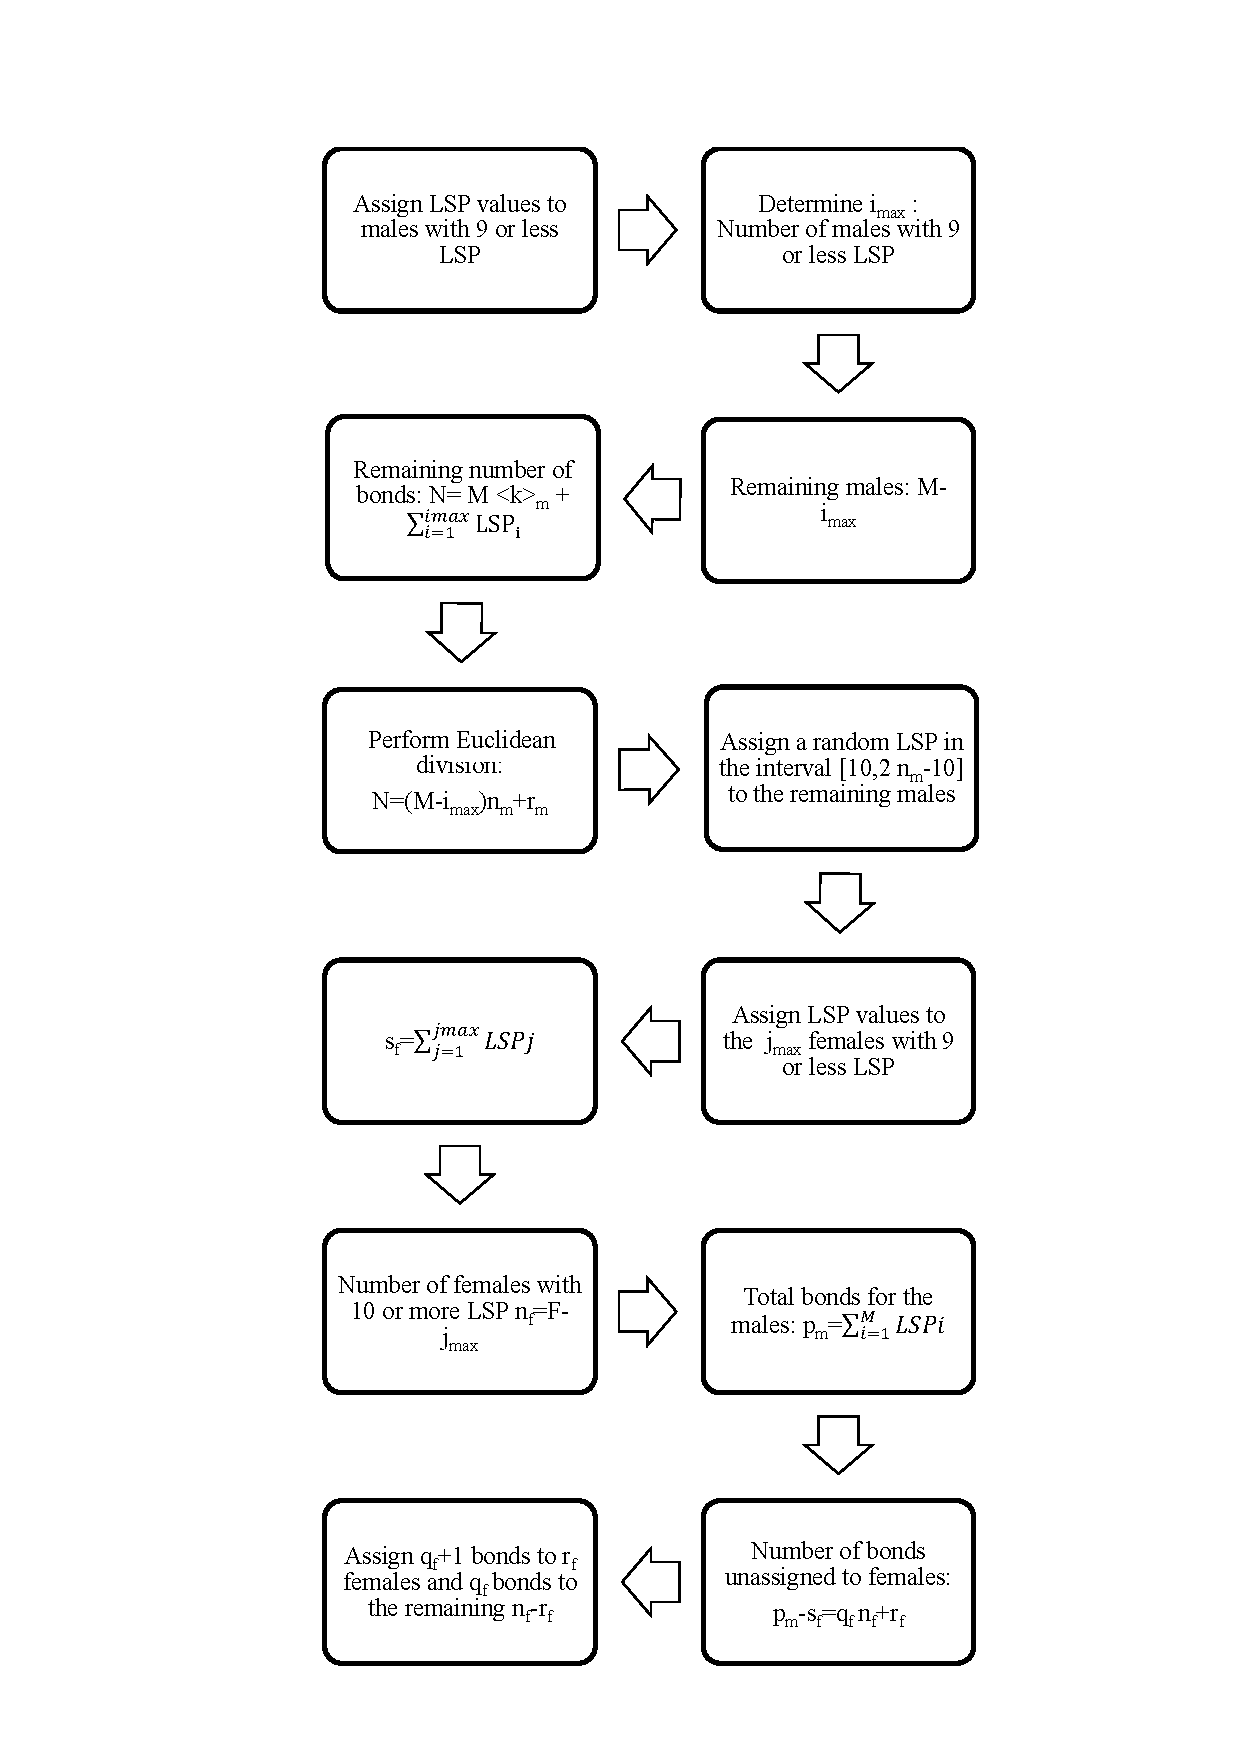
\includegraphics[width=\textwidth]{FluxDiagramI.pdf}
	\end{tabular}
	\caption{Flow diagram for the algorithm corresponding to the assignment of a number of LSPs 
		to every male and female in the network.\label{flux1}}
\end{figure}

These lists will be used to perform the connections of males and females and build the network.
Note that, in Table \ref{table1}, there are more females than males with few LSPs (comparing male and female percentages). It implies that there will be few women with a very large number of LSPs. This fact suggests us to start the assignment procedure with women with the largest LSPs. Otherwise, it would be possible that, when we have to assign LSPs of men to a female with a large number of LSPs, there~will not be enough men with free sexual partners to be assigned and, for this female, it would be impossible to satisfy the condition that the degree of each node was the number of its LSP. 

The assignment of partners was carried out by considering a principle of psychological similarity~\cite{PPS} or assortativity.
Hence, we are going to define a weight function assuming that: women with few LSPs usually match men with few LSPs; people with four or more LSPs use to join with people with four or more LSPs; and couples where one of them has a large number of LSPs and the other few LSPs will be uncommon. Then, for the woman $i$ and the man $j$, we define the following weight~function:

\begin{equation}
\pi(i,j) = 
\begin{array}{l}
\left\lbrace \begin{array}{lc}
| kFemale[i] - kMale[j] | & kFemale[i], kMale[j] \le 4 \\
0 & kFemale[i], kMale[j] > 4 \\
100 & \mbox{otherwise}
\end{array} \right\rbrace, \\
\\
 + | AgeFemale[i] - AgeMale[j] - 1.8 |.
\end{array}
\label{peso}
\end{equation}

The combined weight function, which takes into account the age difference of the partners, $\vert AgeFemale[i] - AgeMale[j] - 1.8 \vert$ is defined in this way because some studies show that the average age difference among the members of a couple in Spain is $1.8$ years \cite{Miret}. 

The MSM population (around a $3.88$ \% of the total male population in Spain) can also be incorporated into the model, but, in this subpopulation, the connectivity would be larger than the heterosexual network.
The MSM population would also be connected with the heterosexual one by links with women in such a way that every MSM individual has a link with a woman with five or more contacts \cite{Calibrate}. The assignment of links is then performed by the {a Greedy Randomized Adaptive Search Procedure (GRASP)} algorithm 
%Pls define. 
%ANSWER: Done.
\cite{greedy,FeoResende}. Details~about the construction of the whole network have been provided in previous studies \cite{Calibrate,Network}. 

\subsection{The Dynamics of HPV Transmission in the Sexual Network}

To implement the simulation of the transmission of HPV among the individuals in the network, a~standard epidemiological model with susceptible and infected states and three types of infections ( {HR, LR} and co-infection) was carried out.
%please define
%ANSWER: It has been defined in the 1st paragraph of the Introduction. If you consider to recall it again, it can be included as follows ".. infections of high risk (HR), low risk (LR) and co-infection ...". 
The epidemiological model is defined by the following parameters:

\begin{itemize}[leftmargin=*,labelsep=5mm]
\item We need some probabilities to determine if a sexual partner is going to produce a contagion of another partner in a given time stage. These parameters are different for each age group:	
 14--17, 18--29, 30--39 and 40--65. Notice that this means that the probability of contagion depends upon the age group of the members of the relationship. Moreover, the probability of connection of these members in the network is also age-dependent
as proposed in Equation (\ref{peso}). The values of these probabilities are determined in the process of the {model} fitting.
%ANSWER: Change "fitting of simulations" by "model fitting".
\item Average time an individual infected by a HR HPV clears the infection and recovers.
\item A similar parameter for clearing the LR HPV infection.
\item If a partner produces the contagion of his/her partner, we need another four parameters to determine if the high or low risk HPV infection is transmitted from man to woman and vice versa. 
\end{itemize}

Another additional parameter is necessary to generate the network. This is the average number of LSPs for men (parameter $k$). Simulations are run by generating a network and carrying out a large number of epidemic evolution time-steps starting with a number of individuals infected by both HPV types as given by the CLEOPATRE study \cite{CLEOPATRE}.
After the warm-up period, we obtain a stable situation and we can proceed with the calibration by comparing the model predictions with real data and deducing the most probable values of the set of parameters.

We have used a calibration procedure using the Particle Swarm Optimization (PSO) algorithm. The prevalence data for each age group is listed in Table \ref{datos}:

\begin{table}[H]
	\centering
	\caption{Prevalence of {HR- and LR}-infected women per age groups from the 
		%Pls define
		%ANSWER:It has been defined in the 1st paragraph of the Introduction. Also, it appears in the list of the abbreviations.	
		CLEOPATRE study \protect\cite{CLEOPATRE}. Co-infections are included in both HR- and LR-infected, mean and $95\%$ confidence intervals.}
	\begin{tabular}{cccc}
		\toprule
		\textbf{Women} & \textbf{HR-Infected} & \textbf{LR-Infected} \\
		\midrule
		18--29 y.o. & $24.10\%,$ $[21.33\%, 26.98\%]$ & $6.36\%,$ $[4.71\%, 8.07\%]$ \\
		30--39 y.o. & $11.01\%,$ $[7.54\%, 15.09\%]$ & $1.26\%,$ $[0.0\%, 3.14\%]$ \\
		40--64 y.o. & $5.96\%,$ $[4.29\%, 7.8\%]$ & $2.37\%,$ $[1.22\%, 3.68\%]$ \\
		\midrule
		18--64 y.o. & $16.23\%,$$[14.52\%, 17.97\%]$ & $4.41\%,$ $[3.42\%, 5.45\%]$ \\
		\bottomrule
	\end{tabular}
	\label{datos}
\end{table}

Note that the network building and the transmission parameters involve randomness and uncertainty due to the random processes used in the network building and the transmission dynamics of the HPV. This fact is going to be taken into account in the  calibration and simulation.

To check the reliability of the model and the calibration, we simulated the HPV vaccination campaign carried out in Australia \cite{Ali}, and compared them with the actual impact published \cite{Ali}. In 2007, Australian health authorities started a vaccination program for 12--13 year-old girls with a~coverage of $73\%$ ($83\%$ in the first dose, $80\%$ in the second dose and $73\%$ in the third dose). In addition, from 2007 to 2009, there was a catch-up vaccination program for women aged 13--26 with a decreasing coverage with age until $52\%$ in women aged 20--26. Their results can be summarized:

\begin{itemize}[leftmargin=*,labelsep=5mm]
\item Two years after the vaccine was introduced, the proportion of GW diagnosed declined by a $59\%$ in vaccine eligible young women aged 12--26 years in $2007$, and by $39\%$ in heterosexual men of the same age.
\item No significant decline was observed in women or men older than $26$ years old, non-resident young women, or men who have sex with men.
\end{itemize}

Two different scenarios were considered to be simulated:

\begin{itemize}[leftmargin=*,labelsep=5mm]
\item Scenario 1: vaccination of $83\%$ of the $14$ year-old girls (or younger girls) plus a catch-up with coverage $73\%$ for 14--26 year-old women.
\item Scenario 2: vaccination of $73\%$ of $14$ year-old girls (or younger girls) plus a catch-up with a~vaccination coverage of $52\%$ for 14--26 year-old women.
\end{itemize}

These simulations represented the upper and lower bounds of the scenario implemented in Australia. The assumed effectiveness of the vaccine was $96.5\%$.

Due to the randomness of the simulations, we will show the average and confidence intervals among the $30$ simulations per every scenario that we have considered above. This number was chosen as a compromise among efficiency of the method and computational feasibility. We have found that, with these runs, we obtain reasonable parameters in many of the simulations. Of course, it would be useful to increase this number, but this cannot be achieved, in a sensible computing time, with the computational resources that we
devoted to the task. For example, a single run takes $162$ hours per run for a network of {$500,000$} nodes 
%ANSWER: Change in the number of nodes to correct figures
and $256$ hours in the case of {$750,000$} nodes
%ANSWER: Change in the number of nodes to correct figures
(in a single processor of a Sandy Bridge platform). Simulations were run on a multi core platform with $64$ processors and $500$ GB RAM and every processor was assigned with the computation of a simulation for a given set of parameters.

\subsection{Calculation of the Number of Infections}

We call $I$ the number of infected women of LR HPV 6 and/or 11 just before the starting of the vaccination campaign; we call $V = ( v_1, \ldots, v_N)$ to the number of infected women of LR HPV 6 and/or 11 every month from the starting of the vaccination program until the end of the simulation. Then,~the~vector 

\begin{equation}
100 \times \left( 1-\displaystyle\frac{v_1}{I}, \ldots, 1-\displaystyle\frac{v_N}{I} \right) \; 
\end{equation}
is a measure of the percentage of decline of number of infected women of LR HPV 6 and/or 11 after the beginning of the vaccination campaign. This will also be applied to men and MSM.

In order to compare GW data given in \cite{Ali} with our model, results referred to infected women of LR HPV 6 and/or 11, we should take into account that, whether a fixed proportion of HPV 6 and/or 11 infected individuals develops warts, the percentage of decline in warts and in infected women of LR HPV 6 and/or 11 will be comparable. 

Another important issue for the natural history of the disease is the persistence of the infection~\cite{AJE2014}. Our model does not consider the persistence ``a priori'', but we derive the cases of genital warts from the number of cases of infected individuals by taking this data into account.

\section{Results}

After calibration, the model predicted an average number of LSPs in men of $7.7$; {confidence interval $95\%$} (CI$95\%$) 
%Pls define.
%ANSWER: done.
$(7.3,8.5)$, with an average duration of an infection due to LR genotypes of $0.5$ CI $95\%$ $(0.3, 0.8)$ years, for men and~women. 

The transmission probability from women for LR genotypes is $0.58$ CI $95\%$ $(0.57, 0.59)$. From men, it is $0.63$ CI $95\%$ $(0.49, 0.72)$. 

\subsection*{The Australian Scenario}

Figure \ref{fig:lrmujeres} shows the percentage of women aged 14--26 infected after starting the vaccination program in both simulated scenarios. The fast decrease in both scenarios can be seen at the very~beginning.
\vspace{-24pt}

\begin{figure}[H]
	\centering
	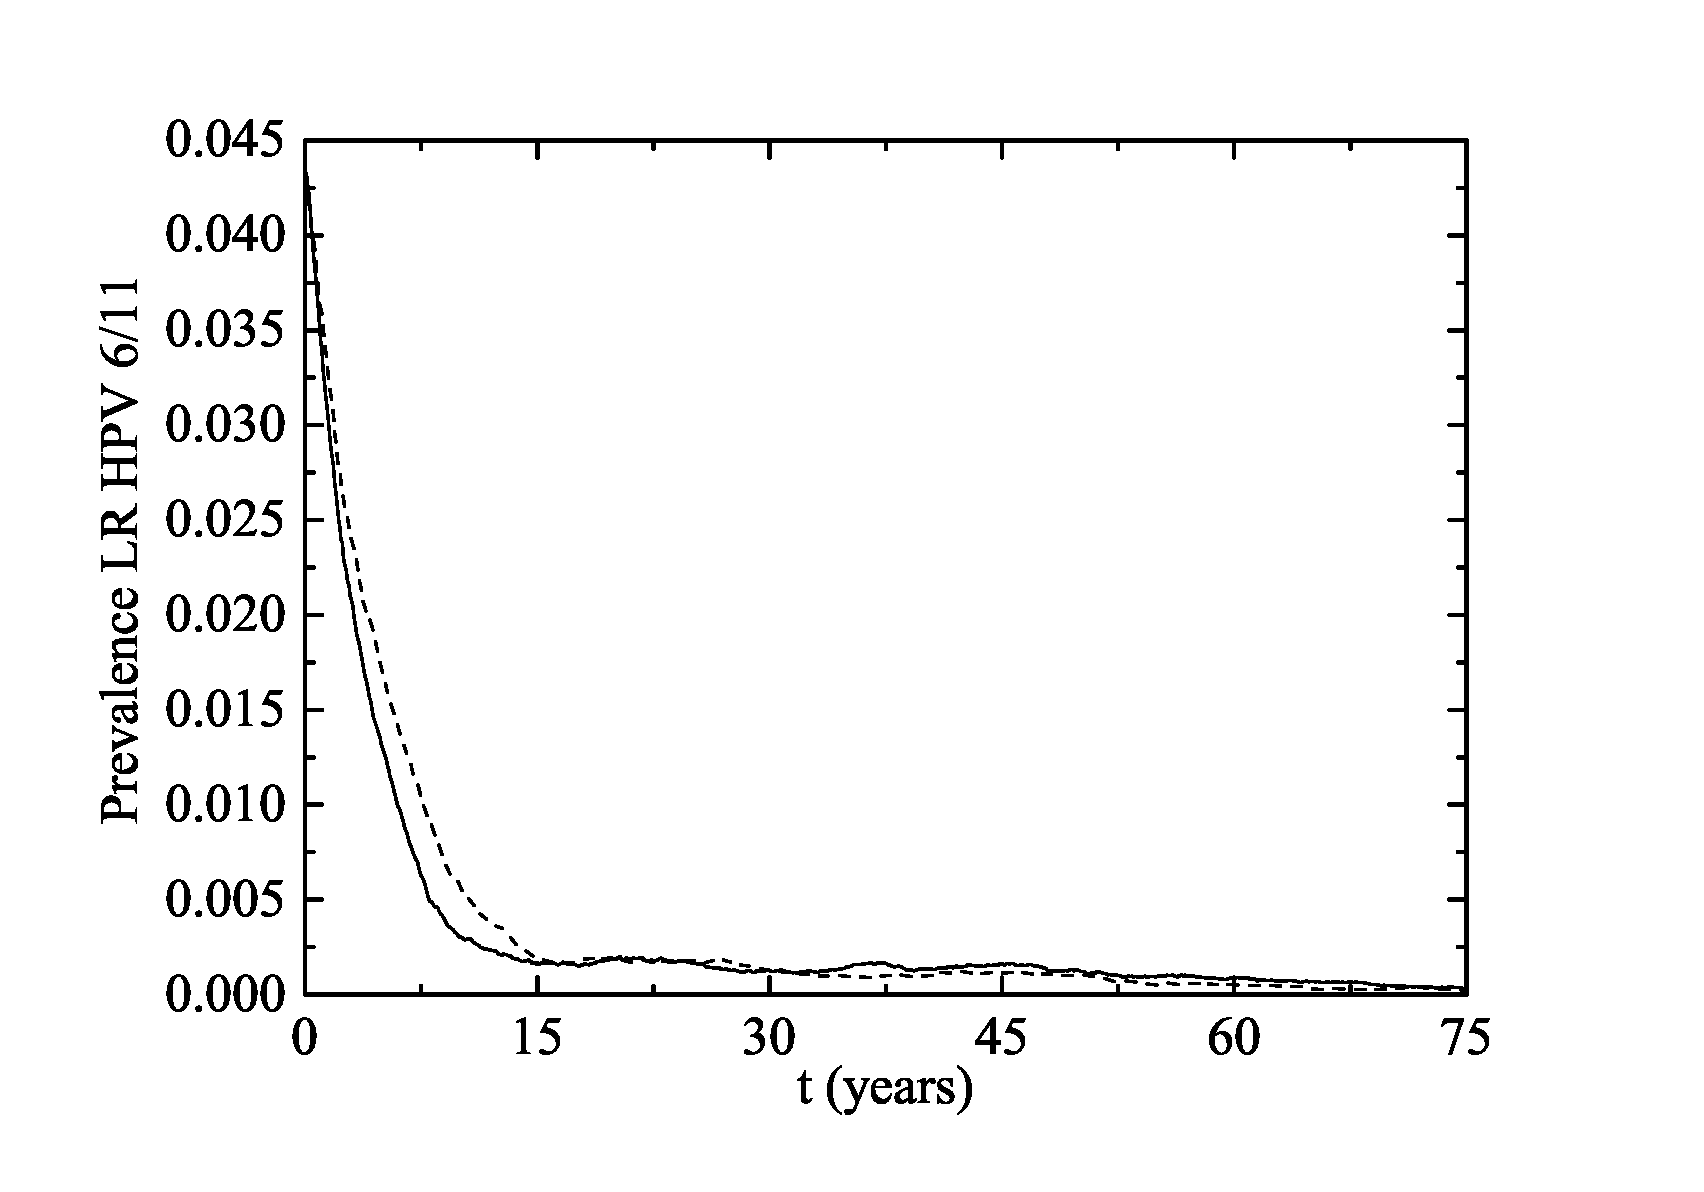
\includegraphics[scale=0.4]{FigLRwomen.pdf}
	\vspace{-12pt}
	\caption{Percentage of women aged 14--26 infected of LR HPV 6 and/or 11 after the 
		%Pls define
		%ANSWER: we did not find anything highlighted	
		implementation of the vaccination program (Scenario 1: solid line and Scenario 2: dotted line).}
	\label{fig:lrmujeres}
\end{figure}

In Figure \ref{fig2}, we have plotted the same data as in Figure \ref{fig:lrmujeres} but from another point of view: the~average percentage of decline of women infected of LR HPV 6 and/or 11. As the vaccination program progresses over time, the percentage of decline obviously grows. 
\vspace{-24pt}

\begin{figure}[H]
	\centering
	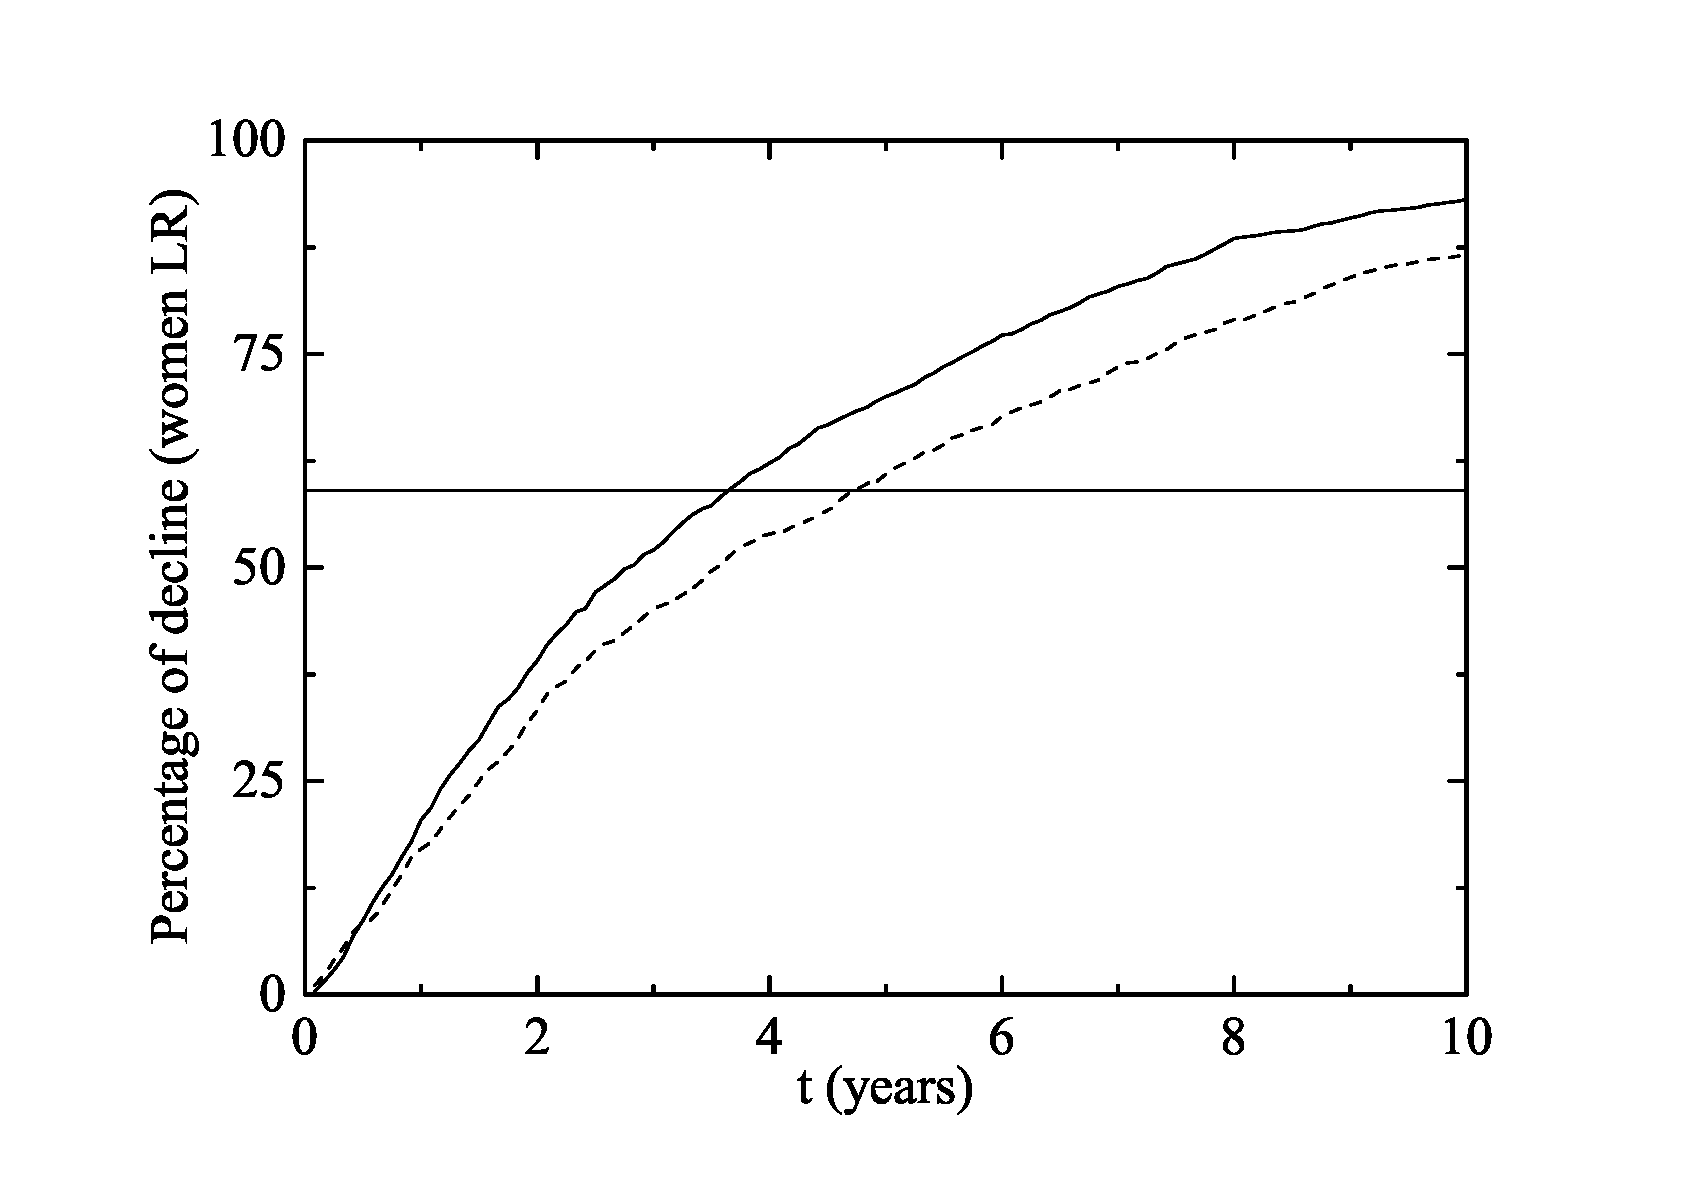
\includegraphics[scale=0.4]{DeclinewomenLR.pdf}
	\vspace{-12pt}
	\caption{Percentage of decline of women aged 14--26 infected of LR HPV 6 and/or 11 (and consequently of GW) after the implementation of the vaccination program in both scenarios (Scenario 1: solid line and Scenario 2: dotted line). The horizontal line represents the percentage of decline in Australian women wart cases after two years.}
	%Pls define. 
	%ANSWER: it is defined in the Introduction, 1st paragraph and GW appears several times along the text. Also, it appears in the list of the abbreviations.
	\label{fig2}
\end{figure}

In our model simulation, after two years of the beginning of the vaccination program, a decline of 33.3--39.1$\%$ has occurred in women and 3.6--4.6 years were necessary to reach the Australian $59\%$ decline rate in GW.

In men aged 14--26 (Figure \ref{fig3}), there was a decline of 23.1--30.5$\%$ after two years and 3--3.75 years were necessary to reach the Australian $39\%$ decline rate of infection. No significant impact on the rate of infection was observed in women or men aged 27--64 in the first $10$ years after the implementation of the vaccination program (Figure \ref{fig4}). It can be explained by the fact that, usually, individuals have sexual intercourses with people more or less the same age.

The herd immunity effect in both scenarios is shown in Figure \ref{fig5} for heterosexual men and  {Figure}~\ref{fig7} for MSM.  Notice that, in men and MSM, any decline is due to herd immunity. The decline of GW in the whole female population is given in Figure \ref{fig6}. This is predicted when the lines representing their decline are over the vaccination line also shown in this figure. We see that the herd immunity effect starts after $2.58$--$2.91$ years when 11.2--14.45$\%$ of women are vaccinated.
%Figure 8 can not appear before Figure 7. Please check. 
%ANSWER: it has been changed to the right place.

Notice that the herd immunity effect is very clear within the $90\%$ CI both for heterosexual men and women, but it is uncertain in the MSM population. In the best case scenario, the MSM subpopulation achieves a large protection level, but there are other situations in which it remains largely unprotected and the HPV strains still circulate among them for many years. This could be attributed to the way in which the MSM individuals are connected: with a very large number of LSPs among them and some casual links with women with large LSPs. If these women, acting like hubs in the network, are~vaccinated, we obtain a fast eradication of the disease in the MSM population and this would be the best scenario.

\begin{figure}[H]
	\centering
	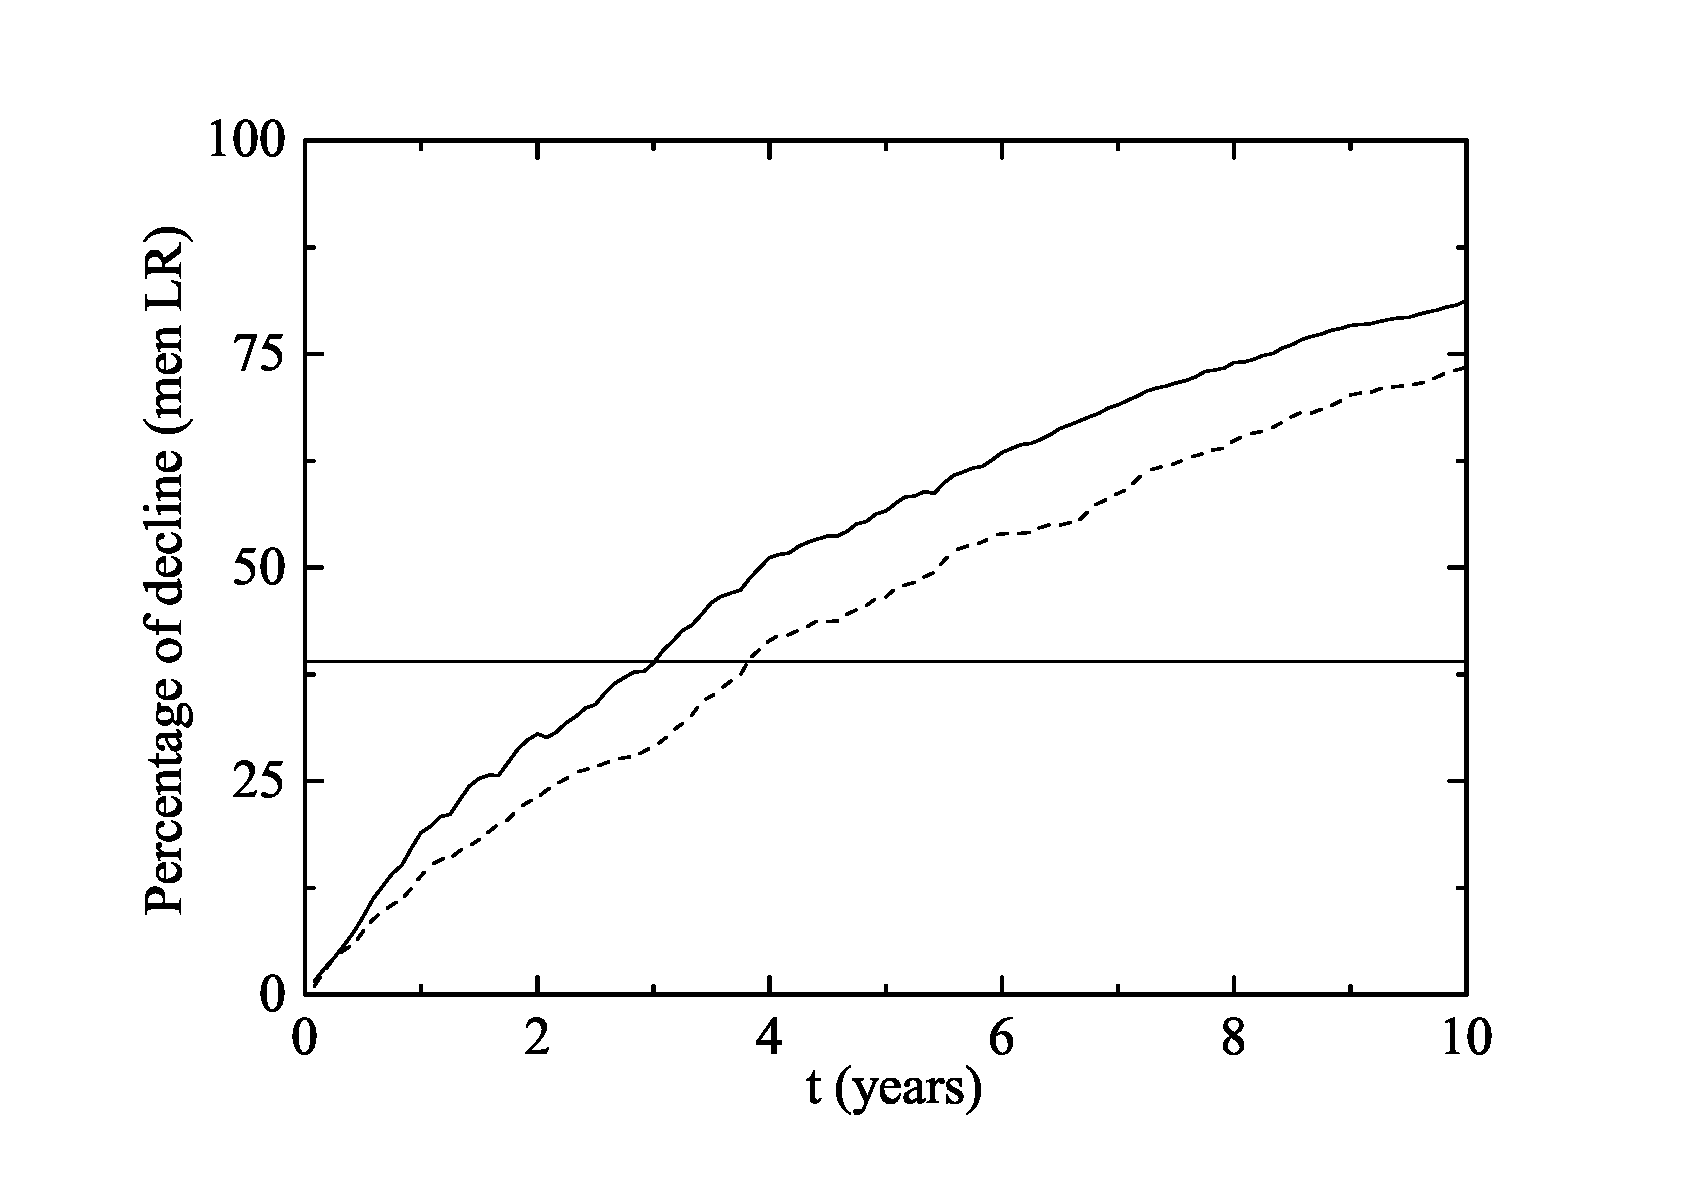
\includegraphics[scale=0.4]{DeclinemenLR.pdf}
	\vspace{-12pt}
	\caption{The same as Figure \protect\ref{fig2} but for men aged 14--26.}
	\label{fig3}
\end{figure}
\vspace{-30pt}

%A simulation of the impact of a program vaccinating 14 years old girls with a coverage of 70\% without catch-up, as for instance, was implemented in Spain, showed that after 2 years the decline in infection in women aged 14-26 with HPV 6 - 11 was about 6\% and 59\% after 8.5 years. On the other hand, the decline in men aged 14-26 infected of HPV 6 - 11 after two years is about 3\% and 39\% after 7.6 years.

%Although this decline refers to infections by HPV 6 and 11 we can expect that it would be very similar for HR HPV genotypes.
\begin{figure}[H]
	\centering
	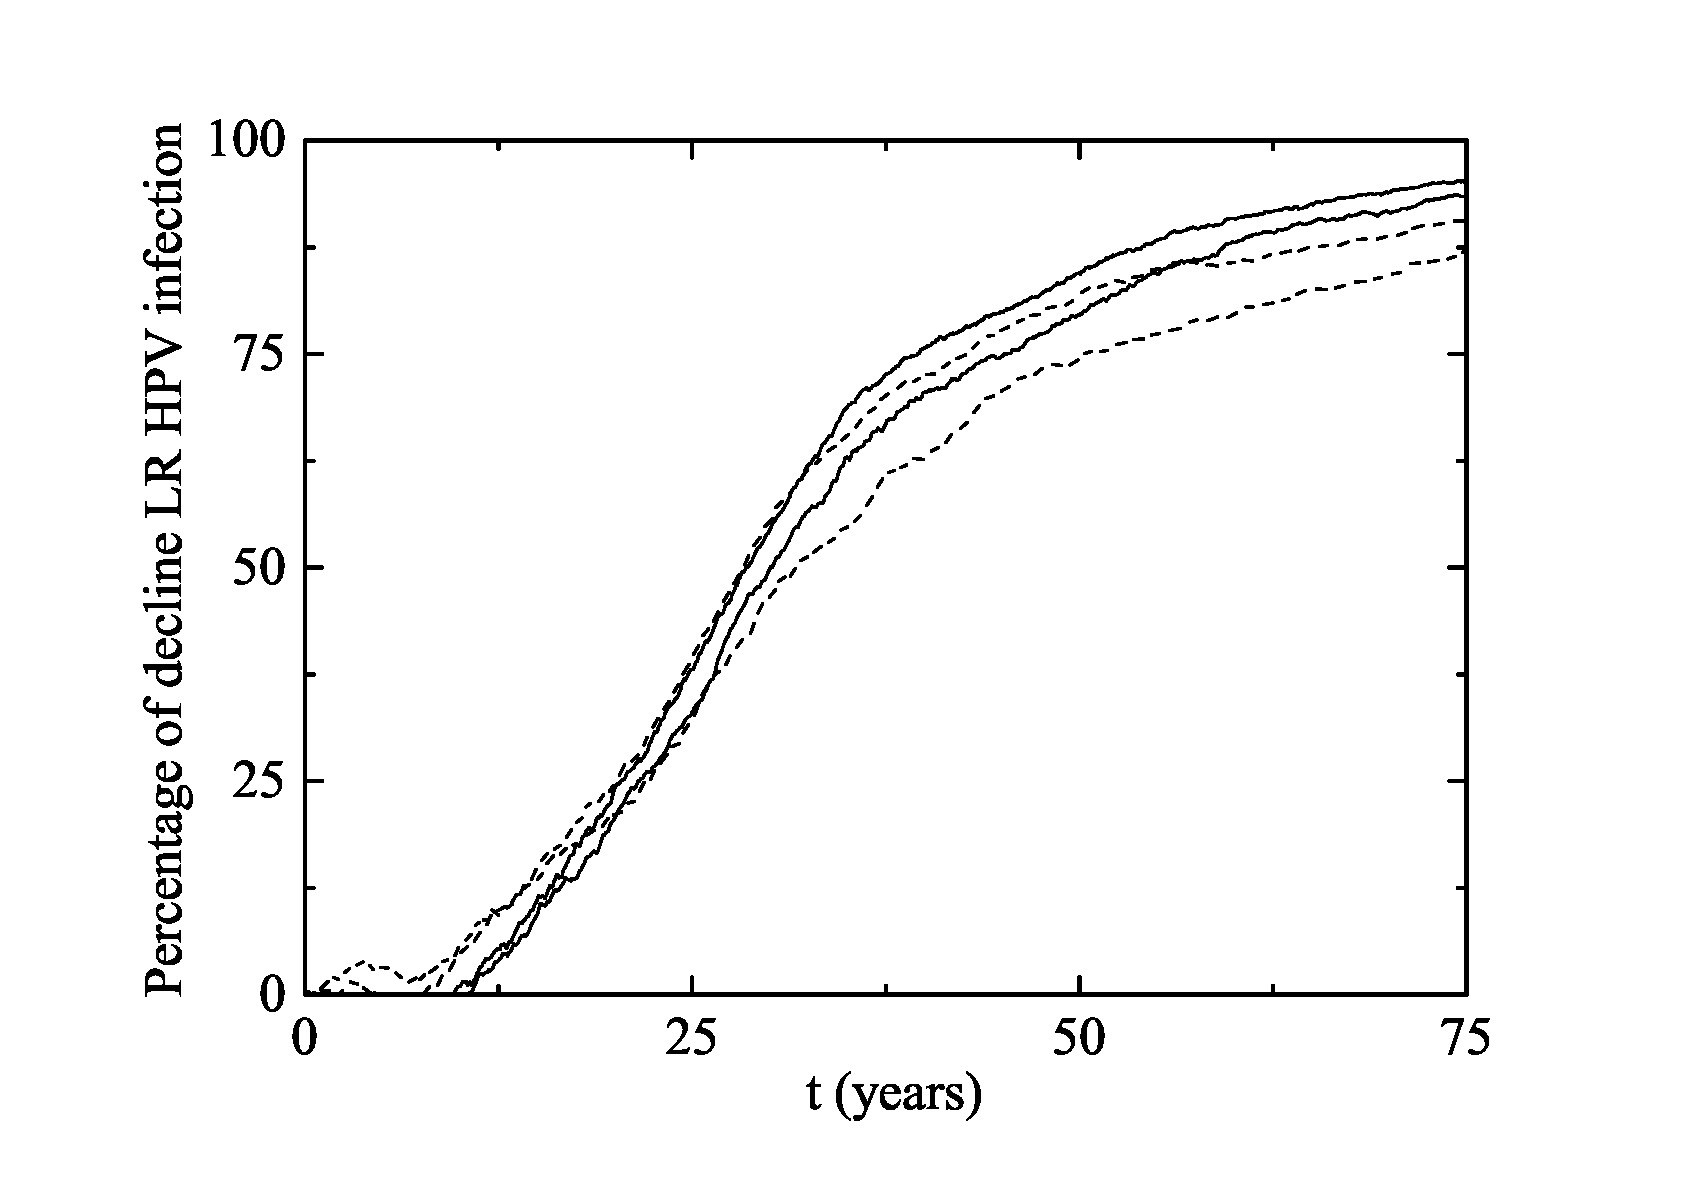
\includegraphics[scale=0.4]{PercentageDeclineolder.pdf}
	\vspace{-12pt}
	\caption{Percentage of decline of men and women aged 27--64 infected of LR HPV 6 and/or 11 (and~consequently of GW) after the implementation of the vaccination program in both scenarios. The~upper solid line corresponds to women in Scenario 1 and the lower solid line corresponds to women in Scenario 2. The upper and lower dotted lines correspond to men in Scenarios 1 and 2, respectively. Notice that no significant decline is observed in women or men aged 27--64 in almost the first 10 years.}
	\label{fig4}
\end{figure}
\vspace{-40pt}

\begin{figure}[H]
	\centering
	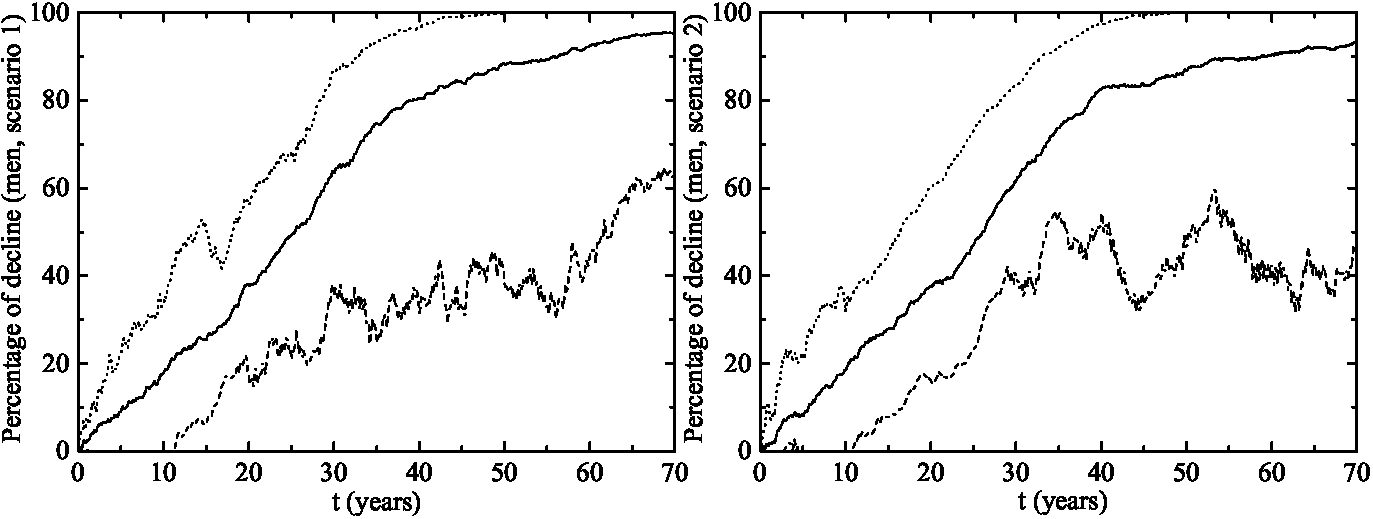
\includegraphics[scale=0.55]{FigHerdImmunity1.pdf}
	\caption{Herd immunity effect of the vaccination program in Australia on heterosexual men (left figure (Scenario 1) and right figure (Scenario 2)). The upper dotted and the lower dashed lines correspond to an interval of 90\% confidence. The solid line
		is the average evolution of the decline in GW.}
	\label{fig5}
\end{figure}
\vspace{-12pt}
\begin{figure}[H]
	\centering
	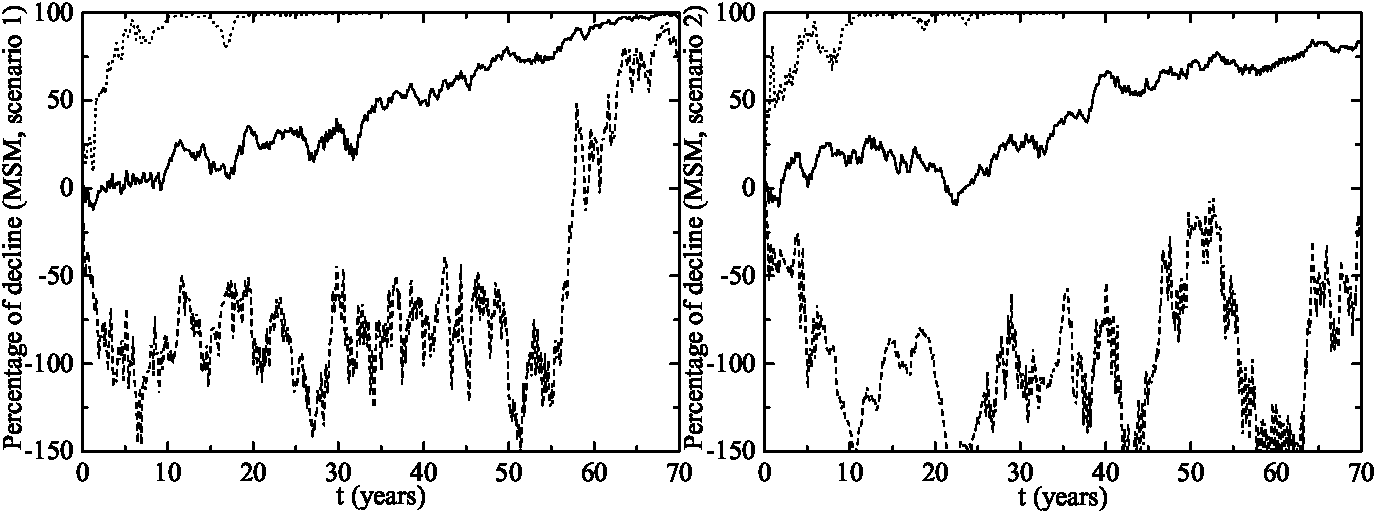
\includegraphics[scale=0.55]{FigHerdImmunity3.pdf}
	\caption{The same as Figure \protect\ref{fig5} but for MSM.}
	%Pls define
	%ANSWER: MSM has been defined in the last paragraph of the Introduction. It is used several times along the text. Also, it appears in the list of the abbreviations.
	\label{fig7}
\end{figure}
\vspace{-12pt}
\begin{figure}[H]
	\centering
	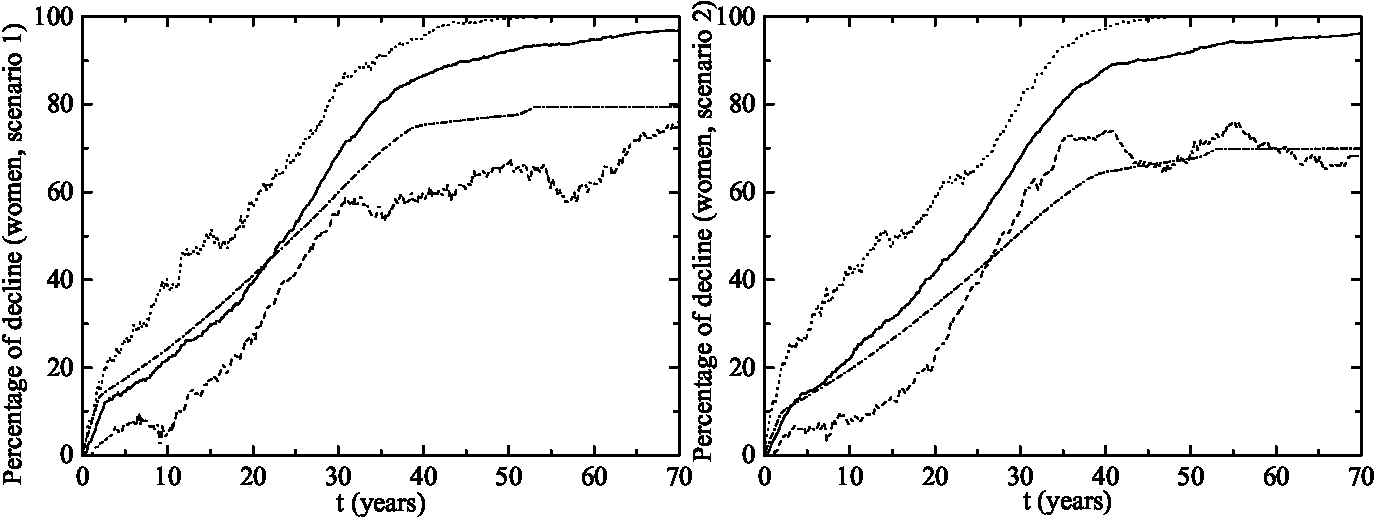
\includegraphics[scale=0.55]{FigHerdImmunity2.pdf}
	\caption{Percentage of decline in GW cases for women for the vaccination program in Australia (left figure (Scenario 1) and right figure (Scenario 2)). The upper dotted and the lower dashed lines correspond to an interval of 90\% confidence. The solid line
		is the average evolution of the decline in GW for the whole female population and the dashed-dotted line is percentage of vaccinated women. Notice~the herd immunity effect also contributes to the decline in the number of infections for unvaccinated women. This can be seen when the decline lines are over the vaccination line.}
	\label{fig6}
\end{figure}

\section{Discussion}

The random network of sexually transmitted HPV including up to $500,000$ nodes was~developed to fit the data of surveys concerning the number of sexual partners throughout life \cite{Calibrate,Network}. Standard~continuous models are insufficient to accurately predict transmission because they do not account for the individual to individual transmission of the infection, the role of hubs in disseminating the virus through the rest of the population and {nor} 
%neither
the vaccination campaigns targeting specific groups of individuals.

This network has successfully been applied to the stable state of infections by LR and HR HPV genotypes in Spain  \cite{Calibrate}. In this study, we mimicked the results found in the HPV vaccination campaign in Australia \cite{Fairley,Ali} and showed very reliable results. 

Model predictions in key epidemiological data was always within the range of the published results. Thus, the $7.7$ number of LSP is close to the $8$ published in Spain \cite{Durex}. In addition, the average duration of infection for LR genotypes is similar to the reported, which is 0.5--1.12 for the LR genotypes~\mbox{\cite{Elbasha1,HPV,Nytray}}. The~transmission probability from women and men is also closed to the parameters used previously~\mbox{\cite{Elbasha1,Nytray}}. All of this reassures the reliability of the model.

Models based upon continuous differential equations predict a slower decrease in the number of infected individuals after implementing similar vaccination campaigns \cite{Elbasha1,Elbasha2}. Hence, the case of the HPV vaccination in Australia provides one of the best real scenarios for testing new network models in mathematical epidemiology. There is an on-going debate on the pertinence of an approach based upon networks on epidemiology \cite{Eubank}, and this work contributes to show the necessity of such an approach in many cases, in particular, in those corresponding to STI.

To validate the model, we used the Australian experience, with two different vaccination coverages: routinely vaccination campaign for 12--13 year-old girls with a coverage of $73\%$ and $83\%$ and a catch-up program in the 14--26 age group with an average coverage of $52\%$ and $73\%$. This~program revealed an important herd effect \cite{Ali}, so that vaccination decreased the incidence of GW even in the non-vaccinated men because of the protection of infection conferred by the vaccine, and the decreased transmission of the virus.

The model predicted a fast decline in the number of infections parallel to the decline in the number of GW in Australia. However, this model was built with Spanish data on sexual behavior \cite{INE} and prevalence of HPV infection \cite{CLEOPATRE}, which might differ to the Australian one, and may explain the minor differences found between the model and the actual data published. Another potential cause of these differences could be the need for a three dose schedule that we simulated, when it has been proposed that with one dose the short term protection against GW is practically $100\%$ \cite{Ali}. Herd immunity in this model of STI is predicted much sooner than in other highly transmitted aerial transported infectious diseases as influenza or  {respiratory syncytial virus}, due to the structure of the network. This supports the need to build
%Pls define. 
%ANSWER: done
appropriate LSP networks.

Other models have also predicted the protection of males by vaccinating girls and women, but~only for heterosexual men, as the model used by Bogaards et al. \cite{Bogaards}. This model uses Bayesian techniques to study the herd immunity effect. However, in contrast with our model, it does not take into account the dynamics of the HPV transmission, the importance of age-groups and the different roles they play in the propagation of these viruses or the links among the MSM subpopulation and the heterosexual network. In this sense, a network model is required to study the impact of the vaccination strategies in short, medium and long time scales.

Vaccination strategies should seek an optimal effectiveness and efficiency. The impact of vaccination in males should always consider the herd immunity of vaccinating girls. However, it is shown that vaccination of women leaves heterosexual males only partially protected at least in the first 10 years after vaccination. However, MSM take 50 years on average, in order to have a decrease in the incidence of infection of $50\%$. This can be the consequence of the large LSP numbers for MSM and their casual connections with women with large LSP numbers in the heterosexual subnetwork.

The model considers a quiet close community, where there is not much contact with other communities. This may not be the case in Spain, which in $2016$ received over $75$ million tourists \cite{INE2}, representing almost double the number of Spanish inhabitants, and when sexual contact is frequent. This may bias the results, as the herd immunity in Spain may not be so clear as in countries with less tourism.

Another issue that we must take into account is the modelling of the population with a high number of contacts because these
individuals are hubs in the network whose vaccination may induce a~faster decline of the virus prevalence. Our approach is rather conservative in the assignment of LSP for men and women with $10$ or more links because we assume that all of them have similar LSP. However, it is expected that individuals with extreme values of LSP are favouring the transmission of HPV in such a way that a targeted vaccination can show its benefit in a very short time.
%el tercer cap�tulo ser� la descripci�n de la situaci�n en Espa�a para HPV LR 
%\chapter{A probabilistic estimation and prediction technique for the evolution of the attitude of the Basque Country population towards ETA}\label{paper3}

This chapter is twofold: on the one hand we are going to use the model developed in Chapter \ref{paper2} to predict the evolution dynamics of the attitude of Basque population towards ETA over the next few years in order to know if the Supporters, the source of ETA members, decrease or not; on the other hand, we introduce a new technique to deal with uncertainty, avoiding some inconveniences detected in the previous chapters, that allows us to give the predictions using confidence intervals.  

Thus, here we propose a computational approach where the data, retrieved from surveys, play a fundamental role to introduce the uncertainty, in estimation and prediction, from the very beginning. 

The chapter is organized as follows. In Section \ref{3.1}, we summarize the model building presented in Chapter \ref{paper2} introducing some variations and the Euskobarometro data since May 2005. In Section \ref{3.2} we propose a technique which will allow us to obtain a set of model parameters that provide $95\%$ confidence intervals for each time instant such that the data uncertainty is captured. We will call this technique \textit{probabilistic estimation}. With the set of parameters obtained in Section \ref{3.2}, in Section \ref{3.3} we obtain a \textit{probabilistic prediction} of the attitude towards ETA of the people of the Basque Country over the next four years. In Section \ref{3.5}, we discuss the results and present the conclusion.

\section{Data and model}\label{3.1}
In Section \ref{2.1} we retrieved data series from the Euskobarometro of November 2012 on the attitude of the Basque Country population towards ETA \cite[Table 20]{eusko}. We gathered the eight different attitudes in only three as we did in the Chapter \ref{paper2}. Data grouped in these three groups appear, in percentages, in Figures \ref{datosS}, \ref{datosR} and \ref{datosA} from May 1995 until Nov 2012. In May 2005 the Spanish Parliament approved the possibility the Government to support dialogue with ETA, what has been considered as a substantial change in the anti-terrorist policy. This policy is still in force and it justifies that we choose this time instant as our model's initial condition. In Table \ref{c3TABLA1} we present the figures in percentages of each subpopulation from May 2005 to Nov 2012.

\begin{table}[h]
\centering
\begin{tabular}{|l|c|c|c|}
\hline
  Survey date  & Support (\%) & Rejection (\%) & Abstention (\%) \\ 
\hline
May 05	&	2	&	93	&	5	\\
Nov 05	&	3	&	93	&	4	\\
May 06	&	3	&	93	&	4	\\
Nov 06	&	4	&	86	&	10	\\
May 07	&	2	&	84	&	14	\\
Nov 07	&	2	&	90	&	8	\\
May 08	&	3	&	90	&	7	\\
Nov 08	&	1	&	93	&	6	\\
May 09	&	4	&	90	&	6	\\
Nov 09	&	3	&	89	&	8	\\
May 10	&	3	&	90	&	7	\\
Nov 10	&	4	&	88	&	8	\\
May 11	&	4	&	90	&	6	\\
Nov 11	&	3	&	89	&	8	\\
May 12	&	5	&	89	&	6	\\
Nov 12	&	3	&	92	&	5	\\
 \hline 
\end{tabular} 
\caption{Percentage of people in the Basque Country with respect to their attitude towards ETA from May 2005 to Nov 2012.}
\label{c3TABLA1} 
\end{table}

In Section \ref{2.2}, we introduced the following system of nonlinear differential equations to describe the evolution of the attitudes towards ETA in the Basque Country over time:

\begin{eqnarray}
A'_1(t) = &  \beta_{21} A_2(t) A_1(t) - \beta_{12} A_1(t) A_2(t) + \beta_{31} A_3(t) A_1(t) - \beta_{13} A_1(t) A_3(t), \nonumber \\
A'_2(t) = &  \beta_{12} A_1(t) A_2(t) - \beta_{21} A_2(t) A_1(t) + \beta_{32} A_3(t) A_2(t) - \beta_{23} A_2(t) A_3(t), \nonumber \\
A'_3(t) = &  \beta_{13} A_1(t) A_3(t) - \beta_{31} A_3(t) A_1(t) + \beta_{23} A_2(t) A_3(t) - \beta_{32} A_3(t) A_2(t). \nonumber
\end{eqnarray} 

Taking $\gamma_{12} = \beta_{12}  - \beta_{21}$, $\gamma_{13} = \beta_{13}  - \beta_{31}$ and $\gamma_{23} = \beta_{23}  - \beta_{32}$, the above system can be simplified as follows

\begin{eqnarray}
A'_1(t) = &  -\gamma_{12} A_2(t) A_1(t) - \gamma_{13} A_3(t) A_1(t), \label{3eq1} \\
A'_2(t) = &   \gamma_{12} A_2(t) A_1(t) - \gamma_{23} A_3(t) A_2(t), \\
A'_3(t) = &   \gamma_{13} A_3(t) A_1(t) + \gamma_{23} A_3(t) A_2(t). \label{3eq3}                           
\end{eqnarray} 

Note that if $\gamma_{ij} > 0$ the net movement of individuals is from $A_i$ to $A_j$. The above system of differential equations can be represented by the diagram of Figure \ref{3Modelo}. 
 
\begin{figure}[h]
 \begin{center}
  \includegraphics[scale=0.7]{IMG/3Modelo2.pdf}\\
  \caption{Graph depicting the model (\ref{3eq1})-(\ref{3eq3}). The circles are the subpopulations and the arrows represent the flow of people who change their attitude towards ETA over the time.}\label{3Modelo}
\end{center}
\end{figure} 

\section{Probabilistic estimation: A computational technique to determine the empirical probabilistic distribution of model parameters}\label{3.2}

Roughly, this technique can be summarised in the following steps:

\begin{enumerate}
\item Assuming a probability distribution for every survey, determine data survey confidence intervals.
\item Use the survey probability distributions to sample data (survey simulations) a large number of times, and we obtain the model parameters that make the model fits the sampled data.
\item Among the obtained sets of model parameters, select the ones for which the model output confidence intervals computed substituting all of them into the model and solving it, are as close as possible of the data survey confidence intervals.
\end{enumerate}

Now, we are going to describe it in detail.

\subsection{Data}
Data in Table \ref{c3TABLA1} correspond to the mean percentage obtained from the Euskobarometro surveys since May 2005 to Nov 2012 \cite[Table 20]{eusko}. In the technical specifications of each survey we can see sample sizes of $1800$ and $1200$ interviews (see column 3 in Table \ref{c3TABLA2}). 

Taking into account that the sample is not the same for each survey, let us assume that the survey outputs are independent. For each one of the $16$ available surveys, let us denote by $X^j=(X_1^j,X_2^j,X_3^j)$, $0\leq X_i^j\leq n_j$, $i=1,2,3$, $j=1,\ldots,16$, a random vector whose entries are $X_1^j = $ Support, $X_2^j = $ Rejection, $X_3^j = $ Abstention and $n_j \in \{1200,1800\}$ is the sample size of survey $j$. These components represent exclusive selections (events) with probabilities

\[
P^j(X_1^j=x_1) = \theta_1^j, P^j(X_2^j=x_2) = \theta_2^j, P^j(X_3^j=x_3) = \theta_3^j, \ j=1,\ldots,16,
\]

where $\theta_1^j$, $\theta_2^j$ and $\theta_3^j$ are the percentages collected in Table \ref{c3TABLA1} for each survey $j$, $j=1,\ldots,16$. We have accepted that each random vector $X^j$ follows a multinomial (trinomial) probability distribution. Therefore, the probability that $X_1^j$ occurs $x_1$ times, $X_2^j$ occurs $x_2$ times and $X_3^j$ occurs $x_3$ times is given by

\[
P_{n_j}^j(x_1,x_2,x_3) = \frac{n_j!}{x_1! x_2! x_3!} (\theta_1^j)^{x_1} (\theta_2^j)^{x_2} (\theta_3^j)^{x_3}, \; j=1,\ldots, 16, 
\]

where $x_1+x_2+x_3=n_j$. The resulting trinomials for each Euskobarometro survey can be seen in the column 4 of Table \ref{c3TABLA2}.

\begin{table}[h]
\centering
\begin{scriptsize}
\begin{tabular}{|c|c|c|c|}
\hline
 & Survey  &Sample &	 Joint trinomial probability function	\\
 & dates	& size	&   \\
\hline
$j=1$	&	$t_{1}=$ May 05	&	$n_{1}=1800$	&	$P_{1800}^{1}(x_1,x_2,x_3) = \frac{1800!}{x_1! x_2! x_3!}0.02^{x_1}0.93^{x_2}0.05^{x_3}$	\\
$j=2$	&	$t_{2}=$ Nov 05	&	$n_{2}=1200$	&	$P_{1200}^{2}(x_1,x_2,x_3) = \frac{1200!}{x_1! x_2! x_3!}0.03^{x_1}0.93^{x_2}0.04^{x_3}$	\\
$j=3$	&	$t_{3}=$ May 06	&	$n_{3}=1800$	&	$P_{1800}^{3}(x_1,x_2,x_3) = \frac{1800!}{x_1! x_2! x_3!}0.03^{x_1}0.93^{x_2}0.04^{x_3}$	\\
$j=4$	&	$t_{4}=$ Nov 06	&	$n_{4}=1200$	&	$P_{1200}^{4}(x_1,x_2,x_3) = \frac{1200!}{x_1! x_2! x_3!}0.04^{x_1}0.86^{x_2}0.1^{x_3}$	\\
$j=5$	&	$t_{5}=$ May 07	&	$n_{5}=1200$	&	$P_{1200}^{5}(x_1,x_2,x_3) = \frac{1200!}{x_1! x_2! x_3!}0.02^{x_1}0.84^{x_2}0.14^{x_3}$	\\
$j=6$	&	$t_{6}=$ Nov 07	&	$n_{6}=1200$	&	$P_{1200}^{6}(x_1,x_2,x_3) = \frac{1200!}{x_1! x_2! x_3!}0.02^{x_1}0.9^{x_2}0.08^{x_3}$	\\
$j=7$	&	$t_{7}=$ May 08	&	$n_{7}=1800$	&	$P_{1800}^{7}(x_1,x_2,x_3) = \frac{1800!}{x_1! x_2! x_3!}0.03^{x_1}0.9^{x_2}0.07^{x_3}$	\\
$j=8$	&	$t_{8}=$ Nov 08	&	$n_{8}=1200$	&	$P_{1200}^{8}(x_1,x_2,x_3) = \frac{1200!}{x_1! x_2! x_3!}0.01^{x_1}0.93^{x_2}0.06^{x_3}$	\\
$j=9$	&	$t_{9}=$ May 09	&	$n_{9}=1200$	&	$P_{1200}^{9}(x_1,x_2,x_3) = \frac{1200!}{x_1! x_2! x_3!}0.04^{x_1}0.9^{x_2}0.06^{x_3}$	\\
$j=10$	&	$t_{10}=$ Nov 09	&	$n_{10}=1200$	&	$P_{1200}^{10}(x_1,x_2,x_3) = \frac{1200!}{x_1! x_2! x_3!}0.03^{x_1}0.89^{x_2}0.08^{x_3}$	\\
$j=11$	&	$t_{11}=$ May 10	&	$n_{11}=1200$	&	$P_{1200}^{11}(x_1,x_2,x_3) = \frac{1200!}{x_1! x_2! x_3!}0.03^{x_1}0.9^{x_2}0.07^{x_3}$	\\
$j=12$	&	$t_{12}=$ Nov 10	&	$n_{12}=1200$	&	$P_{1200}^{12}(x_1,x_2,x_3) = \frac{1200!}{x_1! x_2! x_3!}0.04^{x_1}0.88^{x_2}0.08^{x_3}$	\\
$j=13$	&	$t_{13}=$ May 11	&	$n_{13}=1200$	&	$P_{1200}^{13}(x_1,x_2,x_3) = \frac{1200!}{x_1! x_2! x_3!}0.04^{x_1}0.9^{x_2}0.06^{x_3}$	\\
$j=14$	&	$t_{14}=$ Nov 11	&	$n_{14}=1200$	&	$P_{1200}^{14}(x_1,x_2,x_3) = \frac{1200!}{x_1! x_2! x_3!}0.03^{x_1}0.89^{x_2}0.08^{x_3}$	\\
$j=15$	&	$t_{15}=$ May 12	&	$n_{15}=1200$	&	$P_{1200}^{15}(x_1,x_2,x_3) = \frac{1200!}{x_1! x_2! x_3!}0.05^{x_1}0.89^{x_2}0.06^{x_3}$	\\
$j=16$	&	$t_{16}=$ Nov 12	&	$n_{16}=1200$	&	$P_{1200}^{16}(x_1,x_2,x_3) = \frac{1200!}{x_1! x_2! x_3!}0.03^{x_1}0.92^{x_2}0.05^{x_3}$	\\
\hline 
\end{tabular}
\end{scriptsize} 
\caption{Data for probabilistic model estimation. Date, sample size and joint trinomial probability function of each survey. Using these distributions we will be able to compute their $95\%$ confidence intervals. Also, the model will be fitted with samples of these probability distributions.}
\label{c3TABLA2} 
\end{table}

\subsection{Probabilistic estimation}\label{33.2}
In this section, we are going to sample data survey for each survey, using the joint trinomial distribution set in Table \ref{c3TABLA2}. This will be done a high number of times ($10^4$ times) in order to generate a representative sample for each survey. Every time we sample data survey, we determine the model parameter estimations $\gamma_{12}$, $\gamma_{13}$, $\gamma_{23},$ using the Nelder-Mead optimization algorithm \cite{Nelder, Press} with goodness-of-fit $\chi^2$-test \cite{Groot}. The parameters with $p-$value less than $0.05$ will be rejected. The remainder will be sorted by $p-$value descending order. Selecting some of these model parameter vectors, we will be able to use the model outputs to provide a confidence band determined by the percentiles $2.5$ and $97.5$ ($95\%$ confidence interval) in each time instant. This $95\%$ model confidence band ($95\%$ MCB) is what we call \textit{probabilistic estimation}. Let us describe in detail the procedure.

\begin{enumerate}
\item Compute the quantiles $2.5$ and $97.5$ ($95\%$ CI) of each one of the joint multinomial distributions in Table \ref{c3TABLA2}, $j=1,2,\ldots,16$, for Support, Rejection and Abstention subpopulations, obtaining

\begin{eqnarray}
Q_{2.5}^{support} & = & ( 1.39, 2.08, 2.22, 2.92, 1.25, 1.25, 2.22, 0.50, 2.92, 			\nonumber \\ 
                  &   &   2.08, 2.08, 2.92, 2.92, 2.08, 3.83, 2.08 ), 						\nonumber \\
Q_{97.5}^{support} & = & ( 2.67, 4.00, 3.78, 5.17, 2.83, 2.83, 3.83, 1.58, 5.17, 		\nonumber \\ 
                   &   &   4.00, 4.00, 5.17, 5.17, 4.00, 6.25, 4.00 ),   					\nonumber \\
Q_{2.5}^{reject} & = & ( 91.80, 91.50, 91.80, 84.00, 81.90, 88.20, 88.60, 91.50, 		\nonumber \\ 
                 &   &   88.20, 87.20, 88.20, 86.20, 88.20, 87.20, 87.20, 90.40 ), 		\nonumber \\
Q_{97.5}^{reject} & = & ( 94.20, 94.40, 94.20, 87.90, 86.10, 91.70, 91.40, 94.40, 		\nonumber \\
                  &   &   91.70, 90.70, 91.70, 89.80, 91.70, 90.70, 90.70, 93.50 ), 	\nonumber \\                    
Q_{2.5}^{abstention} & = & ( 4.00, 2.92, 3.11, 8.33, 12.10, 6.50, 5.83, 4.67, 4.67, 	\nonumber \\ 
                 &   &   6.50, 5.58, 6.50, 4.67, 6.50, 4.67, 3.83 ), 						\nonumber \\
Q_{97.5}^{abstention} & = & ( 6.00, 5.17, 4.94, 11.80, 16.00, 9.58, 8.22, 7.33, 7.33,  \nonumber \\
                  &   &   9.58, 8.50, 9.58, 7.33, 9.58, 7.42, 6.25 ).  						\nonumber   
\end{eqnarray}

The $95\%$ CI determined by the above percentiles (they can be seen in Figures \ref{3bandas} and \ref{3bandas2} as vertical segments (error bars)) constitute an approximation of the survey results. Moreover, these $95\%$ CI will be valuable to find the best probabilistic estimation.

\item Let us define the following function of the parameters $\gamma_{12}$, $\gamma_{13}$ and $\gamma_{23}$: 

\begin{itemize}
\item[A)] For given values of $\gamma_{12}$, $\gamma_{13}$ and $\gamma_{23}$ parameters, compute the model output in $t_1=$ May 2005, $t_2=$ Nov 2005, ..., $t_{15}=$ May 2012 and $t_{16}=$ Nov 2012 for the three subpopulations, Support, Rejection and Abstention.
\item[B)] Compare, for each subpopulation, the model output obtained in step (2A) to the data values we will sample in step (3A) using the $\chi^2$-test and obtain a $p-$value for each subpopulation.
\item[C)] Calculate the minimum $p-$value among the three above.
\end{itemize}

\item For $i$ = $1$ to $10^4$

\begin{itemize}
\item[A)] Sample values of all the trinomial distributions in Table \ref{c3TABLA2}. Then, we will have one sample of $16$ surveys with percentages for Support, Rejection and Abstention populations from May 2005 until Nov 2012. Therefore, we will have a set of sampled data as in Table \ref{c3TABLA1}.
 
\item[B)] Find the model parameter values $\gamma_{12}^i$, $\gamma_{13}^i$ and $\gamma_{23}^i$ with the highest $p-$value (maximizing the function defined in steps (2A), (2B) and (2C)). To do that, Nelder-Mead optmization algorithm is used \cite{Nelder, Press} using as a goodness-of-fit the $\chi^2$-test.

\end{itemize}

\item Once the above process is completed, store the obtained parameter values and the $p-$value as the vector     

\[
 ( \gamma_{12}^i, \gamma_{13}^i, \gamma_{23}^i, p-\mbox{value}_i ), \ 1 \leq i \leq 10^4.
\]

\item Reject the model parameters with $p-$value less than $0.05$. In our case, $4990$ out of $10^4$ satisfy this restriction. Then, they are sorted by $p-$value descending order as follows,

\begin{equation}
 ( \gamma_{12}^i, \gamma_{13}^i, \gamma_{23}^i, p-\mbox{value}_i ), \ 1 \leq i \leq 4990. \label{3BF}
\end{equation}

\item For $k$ = $2$ to $4990$

\begin{itemize}
\item[A)] Substitute into the model the parameters $( \gamma_{12}^j, \gamma_{13}^j, \gamma_{23}^j )$, for $j=1,2,\ldots, k$, and compute the model output in $t_1=$ May 2005, $t_2=$ Nov 2005, ..., $t_{15}=$ May 2012 and $t_{16}=$ Nov 2012.  

\begin{itemize}
\item[a1)] Take the $k$ model outputs for Support, Rejection and Abstention at time instant $t_1=$ May 2005 and calculate the corresponding quantiles $2.5$ and $97.5$ ($95\%$ CI).  
\item[a2)] Take the $k$ model outputs for Support, Rejection and Abstention at time instant $t_2=$ Nov 2005 and calculate the corresponding quantiles $2.5$ and $97.5$ ($95\%$ CI).  
\item $\cdots$
\item[a16)] Take the $k$ model outputs for Support, Rejection and Abstention at time instant $t_{16}=$ Nov 2012 and calculate the corresponding quantiles $2.5$ and $97.5$ ($95\%$ CI).  
\end{itemize}

\item[B)] Now, gather the $16$ calculated quantiles $2.5$ for Support, Rejection and Abstention subpopulations and store them sequentially on the vectors $S_{2.5}^k$, $R_{2.5}^k$ and $A_{2.5}^k$, respectively.
\item[C)] Gather the $16$ calculated quantiles $97.5$ for Support, Rejection and Abstention subpopulations and store them sequentially on the vectors $S_{97.5}^k$, $R_{97.5}^k$ and $A_{97.5}^k$, respectively.

\item[D)] Calculate the $p-$values using the $\chi^2$-test to datasets obtained in steps (1), (6B) and (6C) grouped in pairs as follows,

\begin{itemize}
\item[d1)] $Q_{2.5}^{support}$ and $S_{2.5}^k$,
\item[d2)] $Q_{97.5}^{support}$ and $S_{97.5}^k$,
\item[d3)] $Q_{2.5}^{reject}$ and $R_{2.5}^k$,
\item[d4)] $Q_{97.5}^{reject}$ and $R_{97.5}^k$,
\item[d5)] $Q_{2.5}^{abstention}$ and $A_{2.5}^k$,
\item[d6)] $Q_{97.5}^{abstention}$ and $A_{97.5}^k$.
\end{itemize}

Note that, in order to know the parameter values which allow us to define the $95\%$ MCB (probabilistic estimation), we compare percentil vectors obtained by the trinomial sampling to the obtained using the model outputs considering the $4990$ optimal values.
 
\item[E)] Calculate $m_k$ the minimum $p-$value among the six above and build the pair $(k, m_k)$.

\end{itemize}

\item Select the pair $(k, m_k)$ among the $4990$ with the maximum $m_k$.

\end{enumerate}

In our case, the obtained value is $k=77$ with $m_{77}=0.972991$ and consequently the $p$-values corresponding to percentiles $2.5$ and $97.5$ for each subpopulation are greater than $m_{77}$.

Now, we take the $k=77$ set of parameters obtained in the above procedure, compute the model output from $t_1=$ May 2005 to $t_{16}=$ Nov 2012, in jumps of $0.05$ and, in each point, we calculate the percentiles $2.5$ and $97.5$ for each subpopulation ($95\%$ MCB). The result (probabilistic estimation) is depicted in Figure \ref{3bandas} as red continuous lines.

\begin{figure}[h]
 \begin{center}
  \includegraphics[scale=0.6]{IMG/3FIT.pdf}\\
  \caption{Probabilistic estimation. The vertical segments (error bars) correspond to the $95\%$ CI of the simulated data using multinomial distributions appearing in Table \ref{c3TABLA2}. The points in the middle of the segments are the mean values in Table \ref{c3TABLA1}. The continuous lines are the model $95\%$ MCB (probabilistic estimation) obtained with the described procedure. Note that most of the segments cross continuous lines determined by the model, capturing the data uncertainty. Only for Rejection and Abstention subpopulations in time instants Nov 2006 and May 2007 the uncertainty is not captured.} \label{3bandas}
\end{center}
\end{figure}   

The vertical segments (error bars) correspond to the $95\%$ CI of the survey data simulated by multinomial distributions appearing in Table \ref{c3TABLA2}. The points in the middle of the segments are the mean values collected in Table \ref{c3TABLA1}. The continuous lines are the model $95\%$ MCB obtained from the model outputs of the first $k=77$ out of $4990$ sets of model parameters that best fit samples of the multinomial distributions in Table \ref{c3TABLA2}.

\subsection{Probabilistic estimation analysis}
The idea of the probabilistic estimation described in the previous section is to obtain $95\%$ model confidence interval bands (MCB) as close as possible, in the sense of $\chi^2$-test, to $95\%$ CI of the data distributions appearing in Table \ref{c3TABLA2} (vertical segments in Figure \ref{3bandas}). This closeness depends on the model and on the data. 

Looking at the graphics in Figure \ref{3bandas}, we can see that almost all the vertical segments (error bars) cross at least a continuous line indicating that data uncertainty is captured by the model, in particular for Support subpopulation. 

Nevertheless, in Social Sciences the data may be very sensitive to punctual events and these events hardly are captured by the model. This happens if we study the Rejection and Abstention subpopulation graphics, where we can distinguish two parts. The first one, from May 2005 to May 2007, the probabilistic estimation intends to follow the data trajectory but the data uncertainty in Nov 2006 and May 2007 is not captured when sudden jumps appear. As we mentioned in Chapter \ref{ETA} and can also be seen in Figures \ref{datosS}, \ref{datosR} and \ref{datosA}, large jumps in the Rejection population correspond to large jumps in the Abstention population, in the opposite direction. We consider that the jumps in Nov 2006 and May 2007 are due to certain events that occurred from Sep 2006 to May 2007 as: increasing of vandalism acts from Sep 2006 to Dec 2006 linked with young left-wing nationalist groups; Barajas Airport Terminal 4 attack claimed by ETA (Dec 2006); in May 2007 local elections, the left-wing nationalist party EAE-ANV was allowed to present candidates in some villages and cities. In the second part, from Nov 2007 until Nov 2012, the continuous lines capture the data uncertainty.

%It is remarkable to note that the use of $\chi^2$-test in the procedure of the previous section to select the best fittings, allowed us to find $4990$ sets of model parameters for which the model estimation cannot be rejected as explanation of the data representing the studied phenomenon. In fact, we also could select the best (highest $p-$value) among all of them.  

Therefore, even though the estimation for Rejection and Abstention subpopulations do not capture the data uncertainty in two time instants, the three subpopulations capture the remainder and this leads us to consider the model and its probabilistic estimation appropriate to provide a prediction of the evolution of the population's attitude towards ETA over the next four years. 

\section{Probabilistic predictions over the next four years}\label{3.3}
Now, taking the model and the $k=77$ set of parameters obtained in the probabilistic estimation, we are going to give the probabilistic prediction over the next four years by computing the model outputs from Nov 2012 to Nov 2016 and then, obtaining the $95\%$ MCB (model continuous lines). We plot the results graphically in Figure \ref{3bandas2} and some numerical values in Table \ref{c3TABLA3}.

\begin{figure}[h]
 \begin{center}
  \includegraphics[scale=0.6]{IMG/3prediction.pdf}\\
  \caption{Probabilistic prediction. This picture is the  Figure \ref{3bandas} including the predictions over the next four years as $95\%$ MCB (model continuous lines).} \label{3bandas2}
\end{center}
\end{figure} 

\begin{table}[h]
\centering
\begin{small}
\begin{tabular}{|c|c|c|c|c|c|c|}
\hline
Date    & \multicolumn{2}{c|}{Support} & \multicolumn{2}{c|}{Rejection} & \multicolumn{2}{c|}{Abstention} 	\\
		& Mean & $95\%$ CI & Mean & $95\%$ CI & Mean & $95\%$ CI \\
\hline
May 2013 & $  3.10$ & $[  1.54,  4.32]$ & $ 90.69$ & $[ 88.02, 93.38]$ & $  6.22$ & $[  4.52,  9.01]$ \\ 
Nov 2013 & $  2.98$ & $[  1.55,  4.54]$ & $ 90.28$ & $[ 88.11, 93.15]$ & $  6.74$ & $[  4.63,  8.87]$ \\ 
May 2014 & $  2.68$ & $[  1.41,  4.06]$ & $ 90.40$ & $[ 87.87, 92.90]$ & $  6.92$ & $[  4.63,  8.78]$ \\ 
Nov 2014 & $  2.43$ & $[  1.43,  3.88]$ & $ 90.86$ & $[ 88.21, 93.55]$ & $  6.71$ & $[  4.74,  8.90]$ \\ 
May 2015 & $  2.44$ & $[  1.47,  3.84]$ & $ 91.23$ & $[ 89.03, 93.41]$ & $  6.34$ & $[  4.33,  8.66]$ \\ 
Nov 2015 & $  2.62$ & $[  1.42,  4.26]$ & $ 91.22$ & $[ 88.76, 93.25]$ & $  6.17$ & $[  4.60,  8.08]$ \\ 
May 2016 & $  2.72$ & $[  1.42,  4.17]$ & $ 91.01$ & $[ 88.56, 93.39]$ & $  6.27$ & $[  4.49,  8.99]$ \\ 
Nov 2016 & $  2.72$ & $[  1.46,  4.28]$ & $ 90.87$ & $[ 88.13, 93.13]$ & $  6.41$ & $[  4.43,  8.82]$ \\ 
\hline 
\end{tabular} 
\end{small}
\caption{Mean and $95\%$ confidence interval predictions for the coming eight Euskobarometro surveys.}
\label{c3TABLA3} 
\end{table}

Figure \ref{3bandas2} and Table \ref{c3TABLA3} show us that the attitude towards ETA of the population living in the Basque Country will remain fairly stable over the next four years.

\subsection{Robustness of the presented method}
Note that if we run the described procedure again, taking into account that the multinomial sampling is random, we may obtain a different value of $k$, however, the corresponding $m_k$ will be very similar. In fact, we did it two more times obtaining $k=129$ and $k=84$ with $m_k=0.9624$ and $m_k=0.966348$, respectively. The probabilistic estimations in these two new cases are given in Tables \ref{c3TABLA4} and \ref{c3TABLA5}. We can see that the predictions were very similar. This shows the robustness of the proposed method.

\begin{table}[h]
\centering
\begin{small}
\begin{tabular}{|c|c|c|c|c|c|c|}
\hline
Date    & \multicolumn{2}{c|}{Support} & \multicolumn{2}{c|}{Rejection} & \multicolumn{2}{c|}{Abstention} 	\\
		& Mean & $95\%$ CI & Mean & $95\%$ CI & Mean & $95\%$ CI \\
\hline
May 2013 & $  3.08$ & $[  1.48,  4.76]$ & $ 91.02$ & $[ 88.40, 93.44]$ & $  5.90$ & $[  4.42,  8.33]$ \\ 
Nov 2013 & $  3.09$ & $[  1.59,  4.61]$ & $ 90.41$ & $[ 87.90, 93.33]$ & $  6.50$ & $[  4.35,  8.97]$ \\ 
May 2014 & $  2.86$ & $[  1.39,  4.52]$ & $ 90.30$ & $[ 88.05, 92.89]$ & $  6.84$ & $[  4.43,  8.89]$ \\ 
Nov 2014 & $  2.59$ & $[  1.48,  4.22]$ & $ 90.64$ & $[ 88.50, 93.28]$ & $  6.77$ & $[  4.15,  8.71]$ \\ 
May 2015 & $  2.45$ & $[  1.46,  3.86]$ & $ 91.10$ & $[ 88.54, 93.21]$ & $  6.45$ & $[  3.89,  8.53]$ \\ 
Nov 2015 & $  2.51$ & $[  1.56,  3.93]$ & $ 91.35$ & $[ 88.98, 93.31]$ & $  6.14$ & $[  3.67,  8.41]$ \\ 
May 2016 & $  2.67$ & $[  1.47,  4.32]$ & $ 91.28$ & $[ 88.79, 93.33]$ & $  6.05$ & $[  3.56,  8.29]$ \\ 
Nov 2016 & $  2.75$ & $[  1.31,  4.40]$ & $ 91.06$ & $[ 88.09, 93.19]$ & $  6.19$ & $[  3.74,  8.75]$ \\ 
\hline 
\end{tabular} 
\end{small}
\caption{Mean and $95\%$ confidence interval predictions for the coming eight Euskobarometro surveys for the second procedure execution, $k=129$ and $m_k=0.9624$.}
\label{c3TABLA4} 
\end{table}

\begin{table}[h]
\centering
\begin{small}
\begin{tabular}{|c|c|c|c|c|c|c|}
\hline
Date    & \multicolumn{2}{c|}{Support} & \multicolumn{2}{c|}{Rejection} & \multicolumn{2}{c|}{Abstention} 	\\
		& Mean & $95\%$ CI & Mean & $95\%$ CI & Mean & $95\%$ CI \\
\hline
May 2013 & $  3.13$ & $[  1.73,  4.79]$ & $ 90.89$ & $[ 88.29, 93.22]$ & $  5.98$ & $[  4.47,  8.32]$ \\ 
Nov 2013 & $  3.08$ & $[  1.79,  4.59]$ & $ 90.34$ & $[ 87.87, 92.99]$ & $  6.57$ & $[  4.38,  8.81]$ \\ 
May 2014 & $  2.85$ & $[  1.47,  4.61]$ & $ 90.31$ & $[ 88.17, 92.28]$ & $  6.84$ & $[  4.79,  8.89]$ \\ 
Nov 2014 & $  2.56$ & $[  1.47,  4.23]$ & $ 90.66$ & $[ 88.11, 92.88]$ & $  6.78$ & $[  4.79,  8.67]$ \\ 
May 2015 & $  2.39$ & $[  1.50,  3.66]$ & $ 91.12$ & $[ 88.65, 93.34]$ & $  6.50$ & $[  4.27,  8.51]$ \\ 
Nov 2015 & $  2.48$ & $[  1.54,  3.84]$ & $ 91.34$ & $[ 89.30, 93.05]$ & $  6.18$ & $[  4.40,  8.37]$ \\ 
May 2016 & $  2.67$ & $[  1.47,  4.26]$ & $ 91.17$ & $[ 88.63, 93.08]$ & $  6.15$ & $[  4.71,  8.09]$ \\ 
Nov 2016 & $  2.71$ & $[  1.43,  4.35]$ & $ 90.94$ & $[ 87.93, 93.28]$ & $  6.35$ & $[  4.18,  8.69]$ \\ 
\hline 
\end{tabular} 
\end{small}
\caption{Mean and $95\%$ confidence interval predictions for the coming eight Euskobarometro surveys for the third procedure execution, $k=84$ and $m_k=0.966348$.}
\label{c3TABLA5} 
\end{table}

Also, we should say that last June 27th, 2013 was published the Euskobarometro of May 2013 with $1200$ interviews and values given in Table \ref{c3TABLA6}. The $95\%$ confidence intervals of this last Euskobarometro were calculated as in the Step 1 of the procedure described in Section \ref{33.2}.

\begin{table}[h]
\centering
\begin{small}
\begin{tabular}{|c|c|c|c|c|c|c|}
\hline
Date    & \multicolumn{2}{c|}{Support} & \multicolumn{2}{c|}{Rejection} & \multicolumn{2}{c|}{Abstention} 	\\
		& Mean & $95\%$ CI & Mean & $95\%$ CI & Mean & $95\%$ CI \\
\hline
May 2013 & $3$ & $[ 2.08,  4.00]$ & $89$ & $[ 87.17, 90.75]$ & $8$ & $[  6.50,  9.58]$ \\ 
\hline 
\end{tabular} 
\end{small}
\caption{Mean and $95\%$ confidence interval of the Euskobarometro corresponding to May 2013.}
\label{c3TABLA6} 
\end{table}

Comparing data in Table \ref{c3TABLA6} to results in Tables \ref{c3TABLA3}, \ref{c3TABLA4} and \ref{c3TABLA5}, we can see that the data uncertainty in Euskobarometro May 2013 is captured by our predictions in the three tables.

%\section{Simulating policies to reduce the Supporters population}\label{3.4}
%We are assuming that the Supporters population is the source of ETA members (Chapter \ref{ETA}) and, as we see in the previous section, with the current policies the Supporters population will remain fairly stable over the next four years. If the policymakers want to reduce this population in order to accelerate ETA's extinction, they should enforce political measures to modify the parameters $\gamma_{12}$ and $\gamma_{13}$, the ones appearing in the equation (\ref{3eq1}) that influences the variation of the Supporters population.
%
%Thus, let us suppose that the policymakers enforce a law in Jan 2013 such that parameters $\gamma_{12}$ and $\gamma_{13}$ are multiplied by $1.5$ that is, we take $50\%$ more people away from Supporters population or we avoid entering $50\%$ less people to Supporters population than the current policy. We simulate this scenario and some model outputs for the dates when the coming eight Euskobarometro surveys will be published, are given in Table \ref{c3TABLA4}.
%
%\begin{table}[h]
%\centering
%\begin{small}
%\begin{tabular}{|c|c|c|c|c|c|c|}
%\hline
%Date    & \multicolumn{2}{c|}{Support} & \multicolumn{2}{c|}{Rejection} & \multicolumn{2}{c|}{Abstention} 	\\
%		& Mean & $95\%$ CI & Mean & $95\%$ CI & Mean & $95\%$ CI \\
%\hline
%May 2013 & $  2.74$ & $[  1.50,  3.95]$ & $ 89.80$ & $[ 87.03, 92.84]$ & $  7.46$ & $[  5.24, 10.33]$ \\ 
%Nov 2013 & $  1.61$ & $[  0.56,  2.97]$ & $ 90.19$ & $[ 88.08, 93.24]$ & $  8.20$ & $[  4.65, 10.17]$ \\ 
%May 2014 & $  1.08$ & $[  0.52,  2.00]$ & $ 91.99$ & $[ 89.68, 94.27]$ & $  6.93$ & $[  4.16,  8.88]$ \\ 
%Nov 2014 & $  1.19$ & $[  0.68,  2.26]$ & $ 93.30$ & $[ 91.24, 95.26]$ & $  5.51$ & $[  3.79,  7.62]$ \\ 
%May 2015 & $  1.95$ & $[  0.92,  4.03]$ & $ 92.97$ & $[ 89.83, 94.67]$ & $  5.08$ & $[  3.56,  6.81]$ \\ 
%Nov 2015 & $  2.52$ & $[  1.19,  4.09]$ & $ 91.25$ & $[ 87.89, 94.06]$ & $  6.23$ & $[  3.92, 10.31]$ \\ 
%May 2016 & $  2.13$ & $[  0.64,  3.79]$ & $ 90.41$ & $[ 87.74, 93.51]$ & $  7.46$ & $[  5.09, 10.57]$ \\ 
%Nov 2016 & $  1.48$ & $[  0.54,  2.92]$ & $ 91.15$ & $[ 88.20, 94.43]$ & $  7.37$ & $[  4.79,  9.78]$ \\ 
%\hline 
%\end{tabular} 
%\end{small}
%\caption{Simulation of a policy to reduce the Supporters population. Mean and $95\%$ confidence interval predictions at the expected dates of the coming eight Euskobarometro surveys.}
%\label{c3TABLA4S} 
%\end{table}
%
%The figures in Table \ref{c3TABLA4S} indicate that, even though the effort of the new policy, at the end of 2016 we get an average reduction of around $1.5\%$ in the Supporters population (from $3\%$ in Nov 2012 to $1.48\%$ in Nov 2016). This fact links with the idea of Castillo-Ch\'avez \& Song in \cite{Fanatismo} cited in Chapter \ref{CAPINTRO} where they say "... even though the core population is on its way of extinction, it can still experience grow and expand in finite time before it begins to decay". It is clear that this finite time may be long.
%
%Other aspect we should take into account is the fact that it is possible that a minimum critical mass of Supporters must be necessary for ETA's survival. Although its number or percentage is unknown, maybe the simulated policy has achieved a Supporters percentage less than the critical mass and consequently, ETA would be in its way to die out. 

\section{Conclusion}\label{3.5}
In this chapter, it is presented a computational technique to deal with uncertainty (in parameter estimation and output predictions) in dynamic social models based on systems of differential equations. This technique takes data from surveys to introduce the uncertainty into the model from the very beginning and returns $95\%$ model confidence interval bands that capture the data uncertainty and predict what will happen in the near future. 
  
The technique is applied to study the evolution dynamics of the attitude of Basque population towards ETA using the model stated in Chapter \ref{paper2}. Thus, we determine a probabilistic estimation in order to find out if the model captures the Euskobarometro data evolution. We observe that the model captures the data uncertainty only partially from May 2005 to May 2007, but from Nov 2007 the probabilistic estimation improves perceptibly. Anyway, the model estimation is non-rejectable using the $\chi^2$-test. Then, we provide a probabilistic prediction of the attitude towards ETA of the population of the Basque Country over the next four years. Prediction figures indicate stabilization in the evolution of the attitudes towards ETA over the next few years, and therefore stabilization in a hypothetical pool of candidates willing to join the organization in upcoming years. As a result, the presented prediction states that the popular support to the ETA will remain stable, if and when the current scenario does not change.

Additionally, some benefits that can be obtained with this approach are:

\begin{itemize}
\item If we consider the model parameters as random variables, the technique presented here as probabilistic estimation allows the estimation of samples of these model parameters (Steps 3, 4 and 5 of the procedure described in Section \ref{33.2}). This fact is of paramount interest because one of main challenges in modelling real problems using random differential equations is to determine the distribution function of model parameters. Therefore, if we use the probabilistic estimation to obtain some samples of the model parameters, in our case $k=77$ parameter samples, we can use these samples and statistical hypothesis testing or kernel functions in order to find distribution functions of the model parameters. 
\item Other aspect that should be mentioned and it could be interesting for survey prediction estimations is the fact that Table \ref{c3TABLA3} (\ref{c3TABLA4} and \ref{c3TABLA5}) may be considered as an estimation of the results of the coming Euskobarometro surveys (mean and $95\%$ confidence interval). This idea may be applied to this and other type of surveys where a reliable underlying dynamic model can be built. As a consequence, some surveys may not be carried out with the corresponding saving of money. Therefore, we consider that this approach may be an interesting tool for social behavior studies.
\end{itemize}


%y el cuarto la situaci�n en Espa�a para el HPV HR 
%\input{CAP4.tex}

        

%\chapter{Conclusions}
The random network of sexually transmitted HPV including up to $100,000$ nodes, was developed to fit the data of surveys concerning the number of sexual partners throughout life \cite{Acedo2017,DezDomingo2017}. Standard continuous models are insufficient to accurately predict transmission because they do not account for the individual to individual transmission of the infection, the role of hubs in disseminating the virus through the rest of the population and neither the vaccination campaigns targeting specific groups of individuals.

This network has successfully been applied to the stable state of infections by LR and HR HPV genotypes in Spain  \cite{Acedo2017}. In this study we mimicked the results found in the HPV vaccination campaign in Australia \cite{ali2013genital}, and showed very reliable results. 

Models based upon continuous differential equations predict a slower decrease in the number of infected individuals after implementing similar vaccination campaigns \cite{elbasha2007model}. Hence, the case of the HPV vaccination in Australia provides one of the best real scenarios for testing new network models in mathematical epidemiology. There is an on-going debate on the pertinence of an approach based upon networks on epidemiology \cite{Eubank} and this work contributes to show the necessity of such an approach in many cases, in particular, in those corresponding to STD.

To validate the model, we used the Australian experience, with two different vaccination coverages: routinely vaccination campaign for $12-13$ year-old girls with a coverage of $73\%$ and $83\%$ and a catch-up program in the $14-26$ age group with an average coverage of $52\%$ and $73\%$. This program revealed an important herd effect \cite{ali2013genital}, so that vaccination decreased the incidence of genital warts (GW) even in the non-vaccinated men because of the protection of infection conferred by the vaccine, and the decreased transmission of the virus.

The model predicted a fast decline in the number of infections parallel to the decline in the number of GW in Australia with very similar values. However, this model was built with Spanish data on sexual behavior \cite{INE} and prevalence of HPV infection \cite{castellsague2012prevalence}, that might differ to the Australian one, and may explain the minor differences found between the model and the actual data published. Herd immunity in this model of STD is predicted much sooner than in other highly transmitted aerial transported infectious diseases as influenza or RSV, due to the structure of the network. This supports the need to build appropriate LSP networks. 

Other models have also predicted the protection of males by vaccinating girls and women, but only for men, as the model used by Bogaards et al. \cite{bogaards2015direct}. This model uses Bayesian techniques to study the herd immunity effect. However, in contrast with our model, it does not take into account the dynamics of the HPV transmission, the importance of age-groups and the different roles they play in the propagation of these viruses or the links among the MSM subpopulation and the heterosexual network. In this sense, a network model is required to study the impact of the vaccination strategies in short, medium and long time scales.

Vaccination strategies should seek an optimal effectiveness and efficiency. In this case, it can be seen the quick apparition of the herd immunity effect on males and females only vaccinating women. However, the herd immunity effect does not appear in  MSM. This can be the consequence of the large LSP numbers for MSM and their casual connections with women with large LSP numbers in the heterosexual subnetwork.

The model considers a quiet close community, where there is not much contact with other communities. This may not be the case in Spain which in $2016$ received over $75$ million tourists \cite{INEturismo}, representing almost the double of the number of Spanish inhabitants, and when sexual contacts are frequent. This may bias the results, as the herd immunity in Spain may not be so clear as in countries with less tourism.

Another issue that we must take into account, is the modelling of the population with a high number of contacts because these individuals are hubs in the network whose vaccination may induce a faster decline of the virus prevalence. Our approach is rather conservative in the assignment of LSP for men and women with $10$ or more links because we assume that all of them have similar LSP. However, it is expected that individuals with extreme values of LSP are favouring the transmission of HPV in such a way that  a targeted vaccination can show its benefit in a very short time.


\begin{thebibliography}{99}


\bibitem{Pathology}
Sirj\"anen, K.; Sirj\"anen, S. Papillomavirus Infections in Human Pathology. Wiley \& Sons: New York,~2000.

%2
\bibitem{Roberts} Roberts, J.S.C. Vaccine for Genital Warts. In {\em Vaccines for Human Papillomavirus Infections and Anogenital Disease}; Tindle, R.W., Ed.; Medical Intellegence Unit 14, R. G. Landes Company: Austin, TX, USA, 1999.

%3
\bibitem{CLEOPATRE} Castellsagu\'e, X.; Iftner, T.; Roura, E.; Antonio Vidart, J.; Kjaer, S.K.; Bosch, F.X.; Mu�oz, N.; Palacios,~S.; San Martin Rodriguez, M.; Serradell, L.; et al.  Prevalence
and genotype distribution of human papillomavirus infection
of the cervix in Spain: the CLEOPATRE study. {\em J. Med. Virol.} {\bf 2012}, {\em 84}, 947--956, doi:10.1002/jmv.23282.

%4
\bibitem{McNeil} McNeil, C. Who invented the VLP Cervical Cancer Vaccines? {\em J. Natl. Cancer Inst.}
{\bf 2006}, {\em 98}, 433.

%5 
\bibitem{Elbasha1} Elbasha E.H.; Dasbach E.J.; Insinga R.P. Model for assessing human papillomavirus vaccination strategies. {\em Emerg. Infect. Dis.} {\bf 2007}, {\em 13}, 28--41.

%6
\bibitem{Elbasha2} Elbasha, E.H.; Galvani, A.P. Vaccination against multiple HPV types. {\em Math. Biosci.} {\bf 2005}, {\em  197}, 88--117.

%7
\bibitem{Fairley} Fairley, G.; Hocking, J.; Chen, M.; Donovan, B.C. Rapid decline in warts after national quadrivalent HPV vaccine program. In Proceedings of the 25th International Papillomavirus Conference, Malmo, Sweden, 8--14~May 2009. 

%8
\bibitem{Ali} Ali, H.; Donovan, B.; Wand, H.; Read, T.R.H.; Regan, D.G.; Grulich, A.E.;
Fairley, C.K.;  Guy, R.J. Genital~warts in young australians five
years into national human papillomavirus vaccination programme: National surveillance
data. {\em BMJ} {\bf 2013}, {\em 346}, f2032.

%9
\bibitem{Bogaards} Bogaards, J.A.; Wallinga, J.; Brakenhoff, R.H.; Meijer Chris, J.L.M.; Berkhof, J. Direct benefit of vaccinating boys along with girls against oncogenic human papillomavirus: Bayesian evidence synthesis. \textit{BMJ} \textbf{2015}, \textit{350}, h2016. 

%10
\bibitem{RSV} Acedo, L.;  Mora\~no, J.A.; Villanueva, R.J.; Villanueva-Oller, J.; D\'{\i}ez-Domingo, J. Using random networks to study the dynamics of respiratory syncytial virus (RSV) in the Spanish region of Valencia. {\em Math. Comp. Mod.} {\bf 2011},
{\em 54}, 1650--1654.

%11
\bibitem{Obesity} Christakis, N.A.; Fowler, J.H. The Spread of Obesity in a Large Social Network over 32 Years. {\em N. Engl. J.
	Med.} {\bf 2007}, {\em 357}, 370--379.

%12
\bibitem{HPV}  Burchell, A.;  Richardson, H.;  Mahmud, S.M.; Trottier, H.; Tellier, P.P.;  Hanley, J.;  Coutl\'ee, F.;  Franco,~E.L. Modeling the Sexual Transmissibility of Human Papillomavirus Infection using Stochastic Computer Simulation and Empirical Data from a Cohort Study of Young Women in Montreal, Canada. {\em  Am.~J.~Epidemol.} {\bf 2006}, {\em 169}, 534--543.

%13
\bibitem{Web} Liljeros, F.; Edling, C.R.; Nunes, L.A.; Stanley, H.E.;  \r{A}berg, Y. The web of human sexual contacts. {\em Nature} {\bf 2001}, {\em 411}, 907--908.

%14
\bibitem{Bearman} Bearman, P.S.;  Moody, J.; Stovel, K. Chains of Affection: The Structure of
Adolescent Romantic and Sexual Networks. {\em Am. J. Sociol.} {\bf July 2004}, {\em 110}, 44--91.

%15
\bibitem{Likoma} Helleringer, S.; Kohler, H.P. Sexual network structure and the spread of HIV in
Africa: evidence from Likoma Island, Malawi. {\em AIDS} {\bf 2007}, {\em 21}, 2323--2332.

%16
\bibitem{Schmid} Schmid, B.V.; Kretzschmar, M. Determinants of sexual network structure and their impact on cumulative
network measures. {\em PLoS Comput. Biol.} {\bf 2012}, {\em 8}, e1002470.

%17
\bibitem{IVE} Portal estadistico de la Generalitat Valenciana (Statistical Portal of the Government of the Community of Valencia) (2013). Available online: \url{http://www.ive.es} (accessed on 6 March 2017)

%18
\bibitem{INE} Encuesta de Salud y H\'abitos Sexuales 2003. (Health and Sexual Habits Survey 2003). July 2004. Instituto Nacional de Estad\'{\i}stica. Available online:\url{http://www.ine.es} (accessed on 6 March 2017)
%http://www.ine.es/dyngs/INEbase/es/operacion.htm?c=Estadistica_C&cid=1254736176785&menu=resultados&idp=1254735573175

%19
\bibitem{Acedo2013} Acedo, L. Mora\~no, J.-A., Brain oscillations in a random neural network. {\em Math. Comput. Model.}
{\bf April 2013}, {\em 57}, 1768--1772. \url{https://doi.org/10.1016/j.mcm.2011.11.028}

%20
\bibitem{Dorogovtsev} Dorogovtsev, S.N.; Mendes, J.F.F. \emph{Evolution of Networks: From Biological Networks to the Internet and WWW};
Oxford University Press; Reprint edition  Oxford, UK (January 14, 2014).

%21
\bibitem{Watts} Watts, D.J.; Strogatz, S.H. Collective dynamics of small-world networks. \emph{Nature} {\bf 1998}, {\em 393}, 440--442.

%22
\bibitem{USA2} Key Statistics from the National Survey of Family Growth. Available online: \url{http://www.cdc.gov/nchs/nsfg/key\_statistics/n.htm} (accessed on 14 October 2017).

%23
\bibitem{USA} Chandra, A.; Mosher, W.D.; Copen, C. Sexual Behavior, Sexual Attraction, and Sexual
Identity in the United States: Data From the 2006--2008. National Survey of Family Growth, National Health Statistic Reports, No.~36, 3 March 2011. Available online: \url{http://www.cdc.gov/nchs/data/nhsr/nhsr036.pdf}  (accessed on 15 October 2017).

%24
\bibitem{PPS} Gentner, D.; Markman, A.B. Structure mapping in analogy and similarity. {\em Am. Psychol.} {\bf 1997},  {\em 52}, 45--56.

%\bibitem{Munkres} Munkres J. Algorithms for the Assignment and Transportation Problems. {\em Journal of the Society for Industrial and Applied Mathematics} {\bf 1957}, {\em 5(1)}, 32-38.

%25
\bibitem{Miret} Miret, P. La Similitud Entre Los Componentes De Las Parejas J\'ovenes en Espa\~na en la Primera D\'ecada Del 
Siglo XXI.  Cada Vez M\'as Iguales? (The similarity among the Components of Young Couples in Spain in the First Decade of the XXIst Century.  Increasingly Equal?) {\em Revista de Estudios de Juventud} {\bf 2010}, {\em 90}, 225--255. Available online: \url{http://www.injuve.es/sites/default/files/RJ90-16.pdf} (accessed on 15 October 2017).

%26
\bibitem{Calibrate} Acedo, L.; Burgos, C.; Hidalgo, J.I.; S\'anchez-Alonso, V.; Villanueva, R.J.; Villanueva-Oller, J.
Calibrating a~large network model describing the transmission dynamics of the human papillomavirus using a
particle swarm optimization algorithm in a distributed computing environment. {\em  Int. J. High Perform. Comput. Appl.} {\bf 2017}, doi:10.1177/1094342017697862.

%\bibitem{Hartwing} Hartwig S.; Baldauf J. J.; Dominiak-Felden G.; Simondon F.;
%Alemany L.;  de Sanjos\'e S.;  Castellsagu\'e X. Estimation of the epidemiological
%burden of hpv-related anogenital cancers, precancerous lesions, and genital warts in women
%and men in europe: Potential additional benefit of a nine-valent second generation HPV
%vaccine compared to first generation HPV vaccines. {\em Papillomavirus Research} {\bf 2015}, {\em 1}, 90-100.

%27
\bibitem{FeoResende}  Feo, T.A.;  Resende, M.G.C. Greedy Randomized Adaptive Search Procedures. {\em J.  Glob.
	Optim.} {\bf 1995}, {\em 6}, 109--133.

%28
\bibitem{greedy}  Cormen, T.H.; Leiserson, C.E.; Rivest, R.L.; Stein, C. \emph{Introduction to Algorithms}; MIT Press: Cambridge, MA, USA; McGraw-Hill: New York, NY, USA, 1990.

%29
\bibitem{Network} Acedo, L.; Mart\'{\i}, R.; Palmi, F.; S\'anchez-Alonso, V.; Santonja, F.J.;
Villanueva, R.J., Villanueva-Oller, J. Building Lifetime Heterosexual Partner
Networks. In \emph{Modeling Human Behavior.
	Individuals and Organizations};   J\'odar,~L.,  de la Poza, E., Acedo,  L.,  Eds.; Nova Publishers: Hauppauge, NY, USA,  2017;  Chapter 19, pp. 235--251.

%30
\bibitem{AJE2014} Campos, N.G; Burger, E.A.; Sy, S. An Updated Natural History Model of Cervical Cancer: Derivation of Model Parameters. \textit{Am. J. Epidemiol.} \textbf{2014}, \textit{180}, 545--555.

%31
\bibitem{Durex} Estudio de Conducta Sexual Entre Homosexuales; Study of Sexual Behavior among MSM; Technical report, Durex: 2002.
\newline

%32
\bibitem{Nytray} Nyitray, A.G.; Chang, M.; Villa, L.L.;  Carvalho da Silva, R.J.; Baggio, M.L; Abrahamsen, M.;  Papenfuss,  M.;  Quiterio, M.; Salmer\'on, J.;  Lazcano-Ponce, E.; et al.  The Natural History of Genital Human Papillomavirus Among HIV-Negative Men Having Sex With Men and Men Having Sex With Women. \textit{J. Infect. Dis.} \textbf{2015}, \textit{212}, 202--212, doi: 10.1093/infdis/jiv061.

%33
\bibitem{Eubank} Eubank, S.;  Anil Kumar, V.S.; Marathe, M.V.; Srinivasan, A.; Wang, N. Structure of social contact networks and their impact on epidemics. {\em DIMACS Ser. Discrete Math. Theoret. Comput. Sci.} {\bf 2006}, {\em 70}, 181--214.


%34
\bibitem{INE2} Estad\'{\i}stica de movimientos Tur\'{\i}sticos en Fronteras (Statistics of turism in Spain). Press Release from the Instituto Nacional de Estad\'{\i}stica, Spain. Available online: \url{http://www.ine.es/daco/daco42/frontur/frontur1216.pdf} (accessed on 14 October 2017).

\end{thebibliography}

\end{document}
